\documentclass[a4paper,12pt,oneside, bibliography=totoc]
{scrbook}
\usepackage[utf8]{inputenc}

% Schrift und -kodierung
\usepackage[T1]{fontenc}
\usepackage{lmodern}

% Sprache/Silbentrennung
\usepackage[german]{babel} %TODO change to german if desired
\usepackage{booktabs}
\usepackage{amsmath}
\usepackage{floatflt}
\usepackage{float} 
\usepackage{graphicx}
\usepackage{pbox}
\usepackage{algorithmic}
\usepackage{algorithm}
\usepackage{siunitx}
\usepackage[autostyle]{csquotes}
\usepackage{todonotes}

\usepackage[page, title, titletoc, header]{appendix} %prettier appendix



\usepackage[printonlyused]{acronym}
\usepackage{listings} 
\usepackage{subfig}
\lstset{xleftmargin=2em} %Proper indention of listings


\usepackage{tabularx} %For tables
\usepackage{csquotes} %For Quotes





%Footnote Numbering not reset in new chapters
\usepackage{chngcntr}
\counterwithout{footnote}{chapter}


%Remove last point after section/subsections
\renewcommand{\autodot}{}

\usepackage[htt]{hyphenat} %damit texttt noch Linebreaks mit Silbentrennung erzeugt
\newcommand{\code}[1]{\texttt{#1}} %Programmcode im Textfluss in passendem Font ausgeben




   
%Literatur
%Ordering in references checken, vermutlich was mit style=numeric zu tun
\usepackage[
   backend=biber,
   sorting= none,
   firstinits=true,
   date=long,
   urldate=long
]{biblatex}
\addbibresource{database.bib}
%\addbibresource{literatur2.bib}


\usepackage[]{hyperref}

\begin{document}
\frontmatter %roman page numbers





	\titlehead{
	\begin{center}
	   \includegraphics[width=10cm]{figures/unilogo.pdf}\\
	   	Institute of Computer Science, Software Engineering Group
	\end{center}
	}
	\subject{Bachelorarbeit, Masterarbeit}
	\title{Titel der Abschlussarbeit }
	\author{Vorname Nachname\\ Immatrikulationsnummer: 95XXXX} %engl. Matriculation Number

	\date{18.10.2018 \\
	Advisor: Prof. Dr.-Ing. Elke Pulvermüller \\ %Deutsch: Erstebetreuer
	Co-Advisor: Dennis Ziegenhagen, M.Sc.} %Deutsch: Zweitbetreuer
	
	\maketitle
	
	\clearpage
	
	\addchap*{Abstract}
\textbf{Deutsch}
Die Softwaredokumentation ist ein essenzieller Bestandteil der heutigen Softwareentwicklung geworden. Nichtsdestotrotz leidet die Qualität der Dokumentation häufig und viele Entwickler sind nicht motiviert genug, um eine gute Dokumentation zu schreiben. Das Ziel dieser Arbeit ist es, ein Tool zu entwickeln, dass exemplarisch die Dokumentationsqualität in Java-Programmen analysiert und mittels verschiedener Metriken (Anteil dokumentierter Komponenten an allen Komponenten, Flesch-Score, Kohärenz und Nichterwähnung von Randfällen) bewertet. Dieses Tool ist in GitHub Actions eingebunden, um den Entwickler bei einer sehr schlechten Dokumentationsqualität zu warnen und gegebenenfalls Mergevorgänge zu verhindern.

%\linebreak
\bigskip

\noindent
%\bigskip
\textbf{English} 
The software documentation has become an integral part of software development. Nevertheless, the quality of the documentation is often poor and developers are often not motivated to write good documentation. The goal of this thesis is to develop a tool that can analyze the documentation quality of Java applications by applying different metrics (percentage of documented components in all components, Flesch score, coherence, not mentioning the handling of edge cases). This tool will be integrated in GitHub Actions to warn the developer about poor software documentation quality and to prevent a merge if the quality becomes too poor.  

%TODO Bis jetzt nur Osi Abstract, evtl. etwas ausführlicher für Masterarbeit


	\clearpage
	
	\tableofcontents
	\clearpage

	






\mainmatter %switch roman auf arabic page numbers
\chapter{Introduction}
\setcounter{page}{1} %Seitenzahlen hier mit 1 anfangen

	%Include text from other files into the document --> great for structuring
	\label{sec:introduction}

Ein wichtiger Bestandteil der Softwareentwicklung von heute ist die Softwaredokumentation. Dies liegt unter anderem daran, dass die Größe von Softwareprojekten steigt, sodass kein Entwickler das gesamte Programm im Überblick hat und daher zusätzliche Informationen neben dem Code benötigt \cite[S. 1]{StaticAnalysis:AnIntroduction:TheFundamentalChallengeofSoftwareEngineeringisOneofComplexity.}. Nichtsdestotrotz wird die Softwaredokumentation von Entwicklern oft vernachlässigt \cite[S. 83]{Qualityanalysisofsourcecodecomments}.  Die Gründe für schlechte Dokumentation sind vielfältig. Das Schreiben der Dokumentation wird oft als mühevoll empfunden und erfordert Fähigkeiten, die ein Programmierer nichts zwangsläufig hat\cite[S. 70]{AutomaticQualityAssessmentofSourceCodeComments:TheJavadocMiner} \cite[S. 593]{Softwareengineeringandsoftwaredocumentation:aunifiedlongcourse}.  

Die mangelhafte Dokumentation führt dazu, dass nicht nur nachfolgende Entwickler Probleme mit dem Codeverständnis haben, sondern auch der Entwickler eines Moduls nach einer längeren Pause Zeit aufbringen muss, um den Code wieder zu verstehen. \cite[S. 511]{vestdam} Auch für Kunden/Auftraggeber ist eine gute Dokumentation wichtig, da gut dokumentierte Software tendenziell besser wartbar ist und somit mehr Nutzen bringt \cite[S. 83]{Qualityanalysisofsourcecodecomments}\cite[S. 1]{SoftwareDocumentationManagementIssuesandPractices:ASurvey}.


Dass in vielen Fällen die Softwaredokumentation vernachlässigt wird, ist durch viele Studien belegt. Eine Umfrage aus dem Jahr 2002 mit 48 Teilnehmern belegt beispielsweise, dass Anforderungs- oder Spezifikationsdokumente nur selten bei Änderungen am Quellcode angepasst werden. Außerdem finden 54\% der befragten Entwickler  Textverarbeitungsprogramme wie Word für hilfreich, die nicht für Dokumentationszwecke entwickelt wurden.Diese Programme sind leicht zu bedienen und sehr flexibel, aber nicht effizient  \cite[S. 28-29]{TheRelevanceofSoftwareDocumentationToolsandTechnologies:ASurvey}. 

Eine weitere Studie aus dem Jahr 2019 verdeutlicht viele Aspekte aus der vorgenannten Umfrage. Es wurden dabei Daten aus Stack Overflow, GitHub Issues und Pull Requests und Mailing-Listen automatisiert heruntergeladen und dann von den Autoren analysiert, ob und inwieweit mit mangelhafter Softwaredokumentation zu tun haben.  Die Studie liefert klare Indizien dafür, dass die Softwaredokumentation in vielen Fällen nicht komplett, nicht auf dem neuesten Stand oder sogar nicht korrekt ist. Des Weiteren ist die Softwaredokumentation nicht gut nutzbar oder schlecht lesbar, sodass der Vorteil verloren geht\cite[S.1201 -1204]{SoftwareDocumentationIssuesUnveiled}.







\section{Zielsetzung}
Aus diesen Gründen ist eine regelmäßige Rückmeldung über die Dokumentation von hoher Bedeutung. Eine Möglichkeit, dieses Feedback zu geben, sind spezielle Metriken, welche eine numerische Auskunft über die Qualität der Softwaredokumentation liefern. Diese Metriken liefern dem Programmierer eine gute Einschätzung, ob die Softwaredokumentation ausreichend ist oder eine Verbesserung sinnvoll wäre. Da es im Bereich der Softwaredokumentation, verschiedene Metriken gibt, ist es sinnvoll mehrere Metriken zu verwenden. Die Ergebnisse aller Metriken können dann kombiniert werden. Dabei ist es auch ratsam, die Metriken zu gewichten, weil nicht jede Metrik die gleiche Zuverlässigkeit und Relevanz besitzt.

Damit das Feedback über die Softwaredokumentation auch wahrgenommen wird, sollte die Qualität regelmäßig  überprüft werden. Dies kann automatisiert in \ac{CI/CD}-Prozess erfolgen, bei dem Software kontinuierlich getestet und für den Release (z.~dt. Veröffentlichung) vorbereitet werden kann. Durch CI/CD können Unternehmen effizienter und besser Software entwickeln. So konnte die ING NL die gelieferten Function-Points vervierfachen und die Kosten für einen Function-Point auf einen Drittel reduzieren \cite[S. 520]{Vassallo2016}.

Basierend auf diesen Überlegungen soll ein Tool(z.dt. Werkzeug) entwickelt werden. Dieses Tool soll ein gegebenes Software-Projekt analysieren und eine numerische Bewertung darüber abgeben, die eine heuristische Aussage über die Qualität der Softwaredokumentation trifft.  Dabei soll das Tool primär für Javadoc konzipiert werden, allerdings soll während der Entwicklung auch darauf geachtet werden, dass eine Portierung auf eine andere Programmiersprache möglichst einfach wird und die Bewertung der Dokumentation unabhängig von der Programmiersprache funktioniert. Ziel dabei soll es nicht sein, dass jede Komponente (wie z.~B. Methoden oder Klassen) dokumentiert sein muss, sondern dass die wichtigen Komponenten eine gute Dokumentationsqualität haben und somit die Wartung vereinfacht wird. 



\section{Gliederung}
Zur Umsetzung der Bachelorarbeit wird zunächst ein Einblick in das Thema Code-Smell (Kapitel \ref{chapter:code_smell}) gegeben, da schlechte Softwaredokumentation als Code-Smell angesehen werden kann. Anschließend muss der Begriff der Softwaredokumentation genauer definiert werden, da der Begriff so noch sehr unklar ist    (Kapitel \ref{chapter:documentation}). Zudem wird eine Einführung in Javadoc gegeben, da dieses Tool am Ende der Bachelorarbeit hauptsächlich Java und Javadoc verarbeiten soll (Kapitel \ref{chapter:javadoc}). 
Außerdem werden einige verwandte Programme vorgestellt, die ebenfalls die Qualität der Softwaredokumentation analysieren können. Des Weiteren werden einige wissenschaftliche Arbeiten zusammengefasst, die sich ebenfalls mit der Analyse von Softwaredokumentationen beschäftigen.

Um das Programm in dem \ac{CI/CD}-Prozess einzubinden, wird \enquote{GitHub Actions} verwendet. Dieser Service der Plattform GitHub \footnote{\href{https://github.com/}{Github Website (besucht am 07.01.2022)}} ermöglicht es, eigene Programme (oder Programme aus einer großen Auswahl von anderen Programmierern) auf den Quelltext auszuführen.  Diese Programme können dann Fehlermeldungen werfen, wenn es irgendwelche Probleme mit dem Quelltext gibt, sodass der Entwickler darauf aufmerksam wird und die Probleme lösen kann. Mit dieser Plattform ist damit möglich, die Qualität der Softwaredokumentation regelmäßig zu prüfen und bei einer deutlichen Unterschreitung den Entwickler durch Fehlermeldungen zu warnen.  Eine kurze Einführung in GitHub Actions erfolgt in Kapitel \ref{chapter:github_actions}

Danach wird erläutert, wie das Programm entwickelt wurde und welche Herausforderungen zu bewältigen waren. Zunächst muss das Tool die Dateien finden, die vermutlich Softwaredokumentation enthalten und als relevant angesehen werden. Jede dieser Datei muss dann in einzelne Komponenten zerlegt werden, wobei jede Komponente einen Verweis auf ihre Dokumentation (z~B. Javadoc) enthält. Als Komponente im Sinne dieser Bachelorarbeit werden dabei Klassen, Schnittstellen, Methoden und Felder verstanden.

Als nächstes wird beschrieben, wie das Tool zu einer numerischen Bewertung der Qualität der Softwaredokumentation gelangt. Dazu werden verschiedene Metriken angewendet, die in Kapitel \ref{chapter:metrics} erläutert werden. Das Ergebnis jeder Metrik wird dann geeignet aggregiert, damit der Benutzer des Tools eine grobe Einschätzung der Qualität der Dokumentation hat. Beispielsweise kann ein arithmetischer Mittelwert oder ein gewichteter Mittelwert gebildet werden. 

In Anschluss wird in Kapitel \ref{chapter:github_actions_impl}  wird die Einbindung des Tools in GitHub Actions erläutert. Dazu muss das Programm in ein kompakteres Format gebracht werden und in einer separaten Branch in GitHub hochgeladen werden. 

Anschließend soll das Tool mit anderen Tools, die ebenfalls die Dokumentationsqualität bewerten können, verglichen werden. Dazu werden ausgewählte Java-Projekte aus GitHub mit allen Tools analysiert und die Ergebnisse der Tools verglichen. 











\chapter{Problemstellung Softwaredokumentation}
	%Multiple input files for larger chapters are also possible
	\label{sec:background}
In diesen Kapitel soll die Problemstellung der mangelhaften Softwaredokumentation analysiert werden. Hierzu muss zunächst der Begriff \enquote{Softwaredokumentation} definiert werden. Anschließend werden einige Statistiken präsentiert, die zeigen, dass eine mangelhafte Softwaredokumentation ein reales Problem für Entwickler ist. Des Weiteren sollen die Folgen von schlecht dokumentierten Code analysiert werden. Zudem wird in diesem Kapitel die Grundlagen von Javadocs erläutert, welches das Tool später als Grundlage für die Analyse der Dokumentation nutzt. Zuletzt werden noch einige Programme vorgestellt, die unter anderem auch die Dokumentation von Software bewerten können. 

\section{Definition der Softwaredokumentation}
Um den Begriff \enquote{Softwaredokumentation} zu definieren, sollte zunächst der Begriff \enquote{Dokumentation} definiert werden. Das IEEE  definiert diesen Begriff als jede textliche oder bildliche Information, welche Aktivitäten, Anforderungen, Abläufe oder Ergebnisse beschreibt, definiert, spezifiziert, berichtet oder zertifiziert \cite[S. 28]{IEEEStandardGlossaryofSoftwareEngineeringTerminology}. Kurz zusammengefasst beschreibt eine Dokumentation also, wie sich eine Komponente aufgebaut ist oder wie sie sich verhält.

Diese abstrakte Definition lässt sich so auf Softwareentwicklung übertragen. In \cite[S. 125]{Softwaredocumentationandstandards} wird Softwaredokumentation als eine Sammlung von technischen Informationen beschrieben, die für Menschen lesbar sind und die die Funktionen, Benutzung oder das Design eines Softwaresystems beschreiben. So beschreibt der Autor in [], dass die Hauptaufgabe beim Programmieren nicht sein sollte, einen Computer zu erklären, was er machen sollte, sondern anderen Menschen zu erklären, was der Computer machen sollte.

Im Kontext dieser Bachelorarbeit sollen allerdings nur bestimmte Arten der Softwaredokumentation betrachtet werden, da eine umfassende Betrachtung innerhalb der vorgegebenen Zeit nicht möglich ist. Die wichtigste Kategorie im Kontext der Bachelorarbeit sind bestimmte Kommentare im Quelltext eines Programms, die zu den sogenannten Inline-Kommentaren gehören. Diese Kommentare werden wie normale Kommentare erkannt und werden daher nicht Bestandteil des kompilierten Programms. Nichtsdestotrotz haben diese spezifischen Kommentare aber eine bestimmte Struktur, die eine leichte Verarbeitung durch Computerprogramme ermöglicht und gleichzeitig trotzdem für Menschen lesbar bleibt. In vielen Fällen werden diese Kommentare einer bestimmten Komponente zugeordnet, wobei dies oft dadurch geschieht, dass der Kommentar direkt vor dieser Komponente steht.

Andere Möglichkeiten zur Dokumentation, die nur hier kurz erwähnt werden sollen, sind UML-Diagramme, Handbücher und  Readme-Dateien.


\section{Statistiken zu Softwarequalität}
Dass in vielen Fällen die Softwaredokumentation vernachlässigt wird, ist durch viele Studien belegt. Eine Umfrage aus dem Jahr 2002 mit 48 Teilnehmern belegt beispielsweise, dass Anforderungs- oder Spezifikationsdokumente nur selten bei Änderungen am Quellcode angepasst werden. Außerdem verwenden viele Entwickler häufig Programme, die nicht für Dokumentationszwecke entwickelt wurden (z. B Microsoft Word etc.) \cite[S. 28-29]{TheRelevanceofSoftwareDocumentationToolsandTechnologies:ASurvey}. Diese Programme sind leicht zu bedienen und sehr flexibel, verwenden jedoch teilweise proprietäre Dateiformate und sind daher nicht unbedingt effizient.

Eine weitere Studie aus dem Jahr 2019 verdeutlicht viele Aspekte aus der vorgenannten Umfrage. Es wurden dabei Daten aus Stack Overflow, GitHub Issues und Pull Requests und Mailing-Listen automatisiert heruntergeladen und dann von den Autoren analysiert, ob und inwieweit mit mangelhafter Softwaredokumentation zu tun haben.  Die Studie liefert klare Indizien dafür, dass die Softwaredokumentation in vielen Fällen nicht komplett, nicht auf dem neuesten Stand oder sogar nicht korrekt ist. Des Weiteren ist die Softwaredokumentation nicht gut nutzbar oder schlecht lesbar, sodass der Vorteil verloren geht\cite[S.1201 -1204]{SoftwareDocumentationIssuesUnveiled}.
\section{Javadoc}
Javadoc \cite{Javadoc} ist ein Tool zur Generierung von Dokumentationen, das sich als de-facto Standard für Dokumentationen in der Programmiersprache Java etabliert hat \cite[S. 249]{JavadocViolationsandTheirEvolutioninOpen-SourceSoftware}.  Javadoc besteht aus speziellen Java-Kommentaren, die an bestimmten Stellen im Quellcode eingefügt werden und daher bei der Kompilation nicht berücksichtigt werden. Ein Javadoc-Block beschreibt immer ein bestimmtes Modul (z. B. eine Klasse, Methode oder Feld).Es beginnt mit der Zeichenkette \enquote{/**}, wobei die ersten beiden Zeichen \enquote{/*} den Beginn eines mehrzeiligen Kommentars in Java einläuten, und endet mit \enquote{*/}. Zunächst sollte am Anfang des Blocks eine generelle Zusammenfassung der Komponente geschrieben werden. Danach können sogenannte Tags, die mit dem \enquote{@}-Zeichen beginnen, benutzt werden. Diese beschreiben wiederum einen bestimmten Teilbereich einer Komponente. Es ist zudem Konvention, dass jede Zeile in einem Javdoc-Block mit einem Asterisk beginnt. Tabelle \ref{tab:table_javadoc_method} beschreibt einige Tags für Java-Methoden:
\begin{table}[h]
    \centering
    \begin{tabular}{m{4cm}|m{4cm}|m{7cm}}
    Tag & zusätzliche Parameter &Beschreibung\\
    \hline
        @param  & Paramatername & Beschreibt einen Methodenparameter\\
        \hline
         @return & & Beschreibt den Rückgabewert der Methode, sofern er existiert \\
         \hline
         @throws &Exception & Beschreibt welche Exceptions diese Methode werfen kann und möglichst unter welchen Umständen dies passiert \\
           \hline
         @deprecrated & & Falls diese Methode veraltet ist und nicht mehr verwendet werden sollte, kann hier eine Alternative beschrieben werden. \\
           \hline
         
           \hline
         
         
         
         
    \end{tabular}
    \caption{Wichtige Javadoc-Tags}
    \label{tab:table_javadoc_method}
\end{table}
Listing \ref{lst:simple_javadoc} zeigt ein Beispiel für eine  \enquote{gelungene} Verwendung von Javadoc. Zunächst wird der Zweck der Methode beschrieben, anschließend wird jeder Parameter erläutert. Dabei sollte in komplexeren Fällen auch erklärt werden, welche Werte gültig für den Parameter sind. Danach folgt eine Beschreibung des Rückgabewertes, welche am besten auch jeden möglichen Fall abdeckt. Mit \enquote{{@code ...}} kann auf einen Parameter referenziert werden. Mit diesen Informationen kann der Programmierer leicht überblicken, wie eine Methode genutzt werden, sodass die Einarbeitungszeit und die Fehleranfälligkeit reduziert werden kann.  
		\begin{figure}
			\lstinputlisting
			[caption={Beispielhafter Javdoc-Block für einfache Methode},
			label={lst:simple_javadoc},
			captionpos=b,language=java, basicstyle=\footnotesize, tabsize=1, showstringspaces=false,  numbers=left]
			{figures/ternary.java}
		\end{figure}

Auf der offiziellen Oracle-Webseite werden weitere empfehlenswerte Tipps für gute Javadoc-Kommentare gegeben, die hier auszugsweise und ohne besondere Reihenfolge wiedergegeben werden\cite{HowtoWriteDocCommentsfortheJavadocTool}:
\begin{itemize}
    \item Nicht in jeden Fall vollständige Sätze verwenden, aber klar formulieren, was die Aufgabe einer Komponente ist
    \item In der dritten und nicht in der zweiten Person schreiben
    \item Nicht repetitiv sein. Ein Kommentar, der im Wesentlichen nur den Namen einer Komponente wiedergibt, hat keinen Mehrwert
    \item  Beschreibungen von Methoden sollten mit einem Verb beginnen
    \item bei einem Verweis auf das aktuelle Objekt sollte das spezifische \textit{this} statt des allgemeineren \textit{the} verwendet werden
    \item Bezeichner sollten in mit \textit{<code></code>} umschlossen werden, um deutlich zu machen, dass dies eine andere Komponente ist
    \item Der Kommentar sollte eventuelle Unterschiede unter verschiedene Plattformen erläutern
    \item Die Dokumentation sollte erläutern, wie sich die Komponente in Randfällen verhält
    
\end{itemize}
Diese Javadoc-Blöcke können dann von dem gleichnamigen Tool in eine HTML-Datei umgewandelt werden und ermöglichen den Entwicklern damit einen komfortablen Überblick über alle Komponenten eines Moduls. Zudem könne Javadoc-Blöcke ebenfalls HTML-Inhalte besitzen, die dann von Javadoc in die HTML-Datei übernommen werden, sodass der Entwickler beispielsweise Tabellen zur übersichtlichen Präsentation  von Informationen verwenden kann. Abbildung \ref{fig:javadoc_example_screenshot} zeigt, wie eine Methode mittels Javadoc in HTML beschrieben wird. 
\begin{figure}[h]
    \centering
    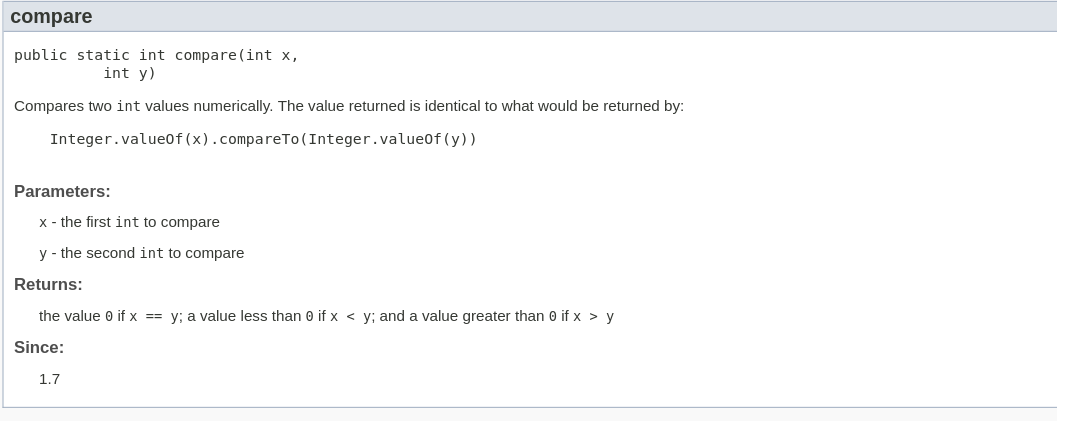
\includegraphics[width=\columnwidth]{figures/javadoc_screenshot.png}
    \caption{Gerenderte HTML-Ausgabe von javadoc}
    \label{fig:javadoc_example_screenshot}
\end{figure}

in Javadoc-Kommentar wird vererbt und muss daher für eine abgeleitete Klasse nicht neu geschrieben oder redundant geklont werden. Dies ist sinnvoll, da abgeleitete Klassen einen Vertrag erfüllen müssen, der bei einer guten Dokumentation auch schon in der Javadoc-Dokumentation beschrieben wird. Auch bei Methoden, die aufgrund einer Schnittstelle implementiert werden müssen, ist eine Neudefinition des Javadoc-Kommentar unnötig. Falls sinnvoll, kann aber dennoch ein eigener Javadoc-Kommentar erstellt werden, der allerdings den Kommentar der Quelle vollständig ersetzt. Mit \textit{@inheritDoc} kann der ursprüngliche Kommentar aber trotzdem eingefügt werden.

Für andere Programmiersprachen gibt es vergleichbare Werkzeuge, die ähnliche Funktionen anbieten und bei denen die Dokumentationen mit einer relativ ähnlichen Syntax erstellt werden. Dazu gehören beispielsweise Doxygen für C++-Programme oder der PHP-Documentor für PHP-Programme. 
\section{Tools zur Bewertung von Javadoc}
Um die Qualität der Softwaredokumentation in Javadoc zu bewerten, gibt es bereits einige Programme. In vielen Fällen handelt es sich dabei um Programme, die nicht auf die Bewertung der Softwaredokumentation beschränkt sind, sondern auch andere Fälle von unsauberem Code erkennen können. Da die Bewertung der Dokumentation nicht der primäre Zweck der Programme ist, sind die verwendeten Metriken recht allgemein und erkennen viele Problemfälle nicht. Nichtsdestotrotz sind diese Programme, dadurch dass sie viele \enquote{Code-Smells} erkennen, sehr gut geeignet, um sich ein gutes Bild über die Qualität des Quellcodes zu verschaffen und den Entwickler zu sauberer Arbeit auch außerhalb von Kommentaren zu ermuntern.
\subsubsection{Checkstyle}
Eines der bekanntesten Programme ist Checkstyle \cite{Checkstyle}. Mit Checkstyle lässt sich beispielsweise prüfen, ob alle Methoden überhaupt ein Javadoc-Block besitzen, der Javadoc-Block korrekt platziert wurde oder ein Javadoc-Tag wie zum Beispiel \enquote{@deprecated} auch mit einer zusätzlichen Begründung versehen wurde. 
\subsubsection{PMD}
Des Weiteren gibt es das Programm PMD\cite{PMD}, das ebenfalls einige Metriken für Javadoc mitliefert. Dazu gehört, ob jede öffentliche Methode dokumentiert wurde oder die Kommentare generell zu lang sind. Interessanterweise gibt es auch die Möglichkeit, bestimmte Wörter, die als anstößig empfunden werden, aus Kommentaren und Dokumentationen auszuschließen, damit Kommentare neutral bleiben. 
\subsubsection{Javadoc}
Das oben erwähnte Javadoc-Tool bietet ebenfalls die Möglichkeit, beim Generieren der HTML-Datei die Qualität des Javadocs zu prüfen. Dabei werden vor allem fehlende Tags für Parameter etc. bemängelt. Zudem erkennt Javadoc auch Tabellen mit fehlender Überschrift und andere Designmängel, die in der HTML-Seite später auffallen. Auch fehlerhaftes HTML kann erkannt werden.

\section{Theoretische Arbeiten im Bereich der Bewertung von Softwaredokumentation}

Neben den praktischen Tools, die den Softwareentwickler bei der Bewertung der Softwaredokumentation unterstützen, wurden auch einige wissenschaftliche Arbeiten veröffentlicht, die sich mit Metriken über Softwaredokumentation auseinandersetzen. 

\subsubsection{JavaDocMiner}
Die wichtigste Arbeit, die eine der Grundlagen dieser Bachelorarbeit ist, ist der \enquote{JavaDocMiner} \cite[S. 68-79]{AutomaticQualityAssessmentofSourceCodeComments:TheJavadocMiner}. In dieser Arbeit wird ein Programm beschrieben, welches mittels einfachen Heuristiken eine Einschätzung der Softwaredokumentation beschrieben. Dabei beschränkt sich der JavaDocMiner nur auf Java-Programme, während das hier zu entwickelnde Tool  auch mit anderen Programmiersprachen zurechtkommen soll.


\subsubsection{iComment}
\enquote{\/\*iComment} \cite[S. 145ff.]{icomment} wurde hauptsächlich für C-Programme entwickelt, um Probleme zwischen der Dokumentation und dem Quellcode zu finden. Dabei konzentriert sich das Programm auf das Finden von Synchronisationsproblemen, die bei Programmen mit mehreren Threads auftauchen können.  Bei einem exklusiven Ausschluss besitzt eine Methode einen sogenannten Lock auf ein Objekt und nur diese Methode darf mit dem Objekt arbeiten.

Setzt nun die Dokumentation einen Lock voraus, aber der Programmierer hat keinen Lock angefordert, können sehr schnelle und subtile Bugs entstehen, die nur schwer findbar sind. 

Das Programm wurde auf dem Quellcode des Linux-Kernels und Mozilla angewandt und dabei mögliche Bugs gefunden, die später auch von den Entwicklern bestätigt wurden\cite[S. 146.]{icomment}.
\subsubsection{@tComment}
Ein anderer Ansatz, der ebenfalls mit Javadoc arbeitet, heißt \enquote{@tComment}\cite[S. 1ff.]{@tComment:TestingJavadocCommentstoDetectComment-CodeInconsistencies}. Dabei wurden die Konsistenz der Javadoc-Dokumentation mit dem tatsächlichen Programmcode verglichen. Anders als die vorherigen Ansätze, wird hier das Programm dynamisch ausgeführt. Dabei werden die verschiedenen Methoden und ihr dazugehörige Javadoc-Dokumentation analysiert und daraus mittels einfacher Heuristiken ermittelt, ob ein  Nullwert für einen Parameter eine Inkonsistenz zwischen Dokumentation und Quellcode offenbart.

Beispielsweise kann die Dokumentation einer Java-Methode beschreiben, dass ein Parameter nicht null sein darf. Daraus kann gefolgert werden, dass ein Nullwert für diesen Parameter zu einer Ausnahme führt. Wenn diese Ausnahme dann auch genauer in der Dokumentation genauer spezifiziert ist, sollte genau diese Ausnahme bei einem Nullwert geworfen werden. 

Falls Nullwerte explizit erlaubt sind, sollte die Methode sich dann stets korrekt verhalten und keine Ausnahmen werfen. 

\enquote{@tComment} kann mit diesen einfachen Regeln jede Methode ausführen und prüfen, ob sich die Methode tatsächlich verhält, wie die Dokumentation es beschreibt. Dabei verwendet das Programm einfache \ac{NLP}-Heuristiken in der englischen Sprache; zum Beispiel prüft das Programm, ob die kurz vor dem Wort \enquote{null} ein negierendes Wort wie \enquote{not} oder \enquote{never} auftaucht und klassifiziert dann den dazugehörigen Parameter als Parameter, der nie null sein darf. 


\section{GitHub Actions}
\subsection{Einführung}
Github Action \cite{GithubActions} ist eine von GitHub angebotene Plattform zur Vereinfachung des \ac{CI/CD}'s. Mithilfe von  Github Actions wird Programmcode ausgeführt, wenn ein bestimmtes Ereignis stattfindet. Dieses Ereignis kann z. B. ein Push-Ereignis sein, bei dem neuer Quellcode in das GitHub-Repository hochgeladen wird, oder eine neue Version des Programms zum Release freigegeben wird. Der Programmcode kann auf einem von GitHub vorbereiteten System ausgeführt werden; es ist aber auch möglich sein eigenes System dafür zur konfigurieren. Schlägt der Programmcode fehl, weil zum Beispiel ein Fehlercode ungleich null zurückgegeben wird oder ein anderer Systemfehler vorliegt, kann der Nutzer sich leicht über den Fehler informieren, indem auf die \enquote{Actions}-Registerkarte klickt. Dort kann der Nutzer auch sämtliche Ausgaben des Programms ansehen, die auf der Konsole ausgegeben werden. Die folgende nummerierte Liste beschreibt grob, wie Programmcode in Github Actions ausgeführt werden kann:
\begin{enumerate}
    \item Ein Ereignis tritt ein, indem beispielsweise neuer Programmcode mittels Push hochgeladen wird 
    \item Github wählt ein geeignetes System aus (z. B. eine virtuelle Maschine oder ein vom Programmierer hierfür konfiguriertes System
    \item Auf dem System wird der aktuelle Programmcode des Repositorys geklont (die Branch kann frei bestimmt werden) 
    \item Der Programmcode ausgeführt, dabei steht der Pfad zum geklonten Repository über die Umgebungsvariable \textit{\$GITHUB\_WORKSPACE} bereit
    \item Abhängig vom Erfolg der Ausführung des Programmcodes:
    \begin{enumerate}
        \item Bei einem Erfolg wird der Programmierer mittels eines grünen Häkchens informiert
        \item Bei einer Fehlermeldung wird der Programmierer mittels eines roten Kreuzes über den Fehlschlag informiert und hat auch Zugriff auf die Fehlermeldungen. Je nach Einstellung des Repositorys können bestimmte Aktivitäten dann auch gestoppt werden, damit fehlerhafter Programmcode nicht weiter verbreitet wird. 
    \end{enumerate}
\end{enumerate}

Ein Anwendungsfall von GitHub Actions sind automatisierte Tests. Bei einem Push-Ereignis kann der aktuelle Programmcode mit einer geeigneten Testbibliothek getestet werden, sodass im Falle eines fehlgeschlagenen Tests der Programmierer informiert wird und die notwendigen Änderungen veranlassen kann. 

\subsection{Wichtige Begriffe im Zusammenhang mit Github Action}
In der folgenden Auflistung werden einige wichtige Begriffe erläutert, die im Zusammenhang mit GitHub Actions verwendet werden und deren Kenntnis zum Verständnis wichtig ist. 
\begin{description}
    \item[Workflow] Ein Workflow(Ablauf) ist eine automatisierter Prozess, der verschiedene Jobs ausführt, wenn ein Ereignis eintritt. Der Worklflow wird durch eine YAML-Datei definiert
    \item[Job] Ein Job ist eine Ansammlung von sogenannten \enquote{Steps}, die man als Befehle interpretieren kann. Alle Befehle in einem Job werden auf der gleichen Maschine ausgeführt. Alle Jobs in einem Workflow werden standardmäßig parallel ausgeführt, da keine Abhängigkeit zwischen den Jobs vermutet wird.
    \item[Step] Ein Step(Schritt) ist ein Shell-Befehl oder ein Verweis auf eine andere GitHub Action, die von einem Job ausgeführt werden soll. Innerhalb eines Jobs werden die Steps in der definierten Reihenfolge ausgeführt. 
    \item[Action] Eine Action ist ein Programm, das in Workflows eingebunden werden kann und häufig vorkommende Aufgaben erledigt. Dies hat den Vorteil, dass Redundanz vermieden wird. Im offiziellen Marketplace von GitHub lassen sich zu vielen verschiedenen Aufgaben bereits Actions finden. Es können aber auch eigene Actions definiert werden, was weiter unten beschrieben wird. 
    \item[Runner] Als Runner wird das System bezeichnet, auf dem die Jobs ausgeführt werden. Dies ist standardmäßig ein Linux-Betriebssystem; es können aber auch Windows oder macOS zur Ausführung des Codes verwendet werden. Bei besonderen Anforderungen kann der Runner auch auf einem System laufen, auf dem der Programmierer selbst Zugriff hat.
\end{description}
\subsection{Erstellung eines Workflows}
Ein Workflow kann über die registerkarte \enquote{Actions} erstellt werden und wird intern in dem Verzeichnis \textit{.github/workflows} gespeichert. Abbildung \ref{lst:simple_workflow} illustriert eine typische Workflow-Datei, die standardmäßig erstellt wird. Der Code wird in Tabelle \ref{tab:descr_example_workflow} genauer erklärt.
\clearpage
\begin{table}[h!]
    \centering
    \begin{tabular}{c|m{10cm}}
        Zeile(n) &  Beschreibung \\\hline
         1 & Der Name des Workflows\\\hline
         2-6 & Hier werden die verschiedenen Ereignisse beschrieben, die den Workflow auslösen. Außerdem werden die Branches spezifiert, die auf das Ereignis überwacht werden sollenö\\\hline
         7 &  Dies erlaubt, dass ein Workflow auch manuell angestoßen wird, etwa zu Debugging-Zwecken\\\hline
         8-9 & Erstellt einen Job mit den Namen \enquote{Build}\\\hline
         10 & Bestimmt auf welchen System der Workflow läuft\\\hline
         11 & Beginnd er einzelnen Steps\\\hline
         12 & Bestimmt, das der Quellcode des Repositorys geklont wird und dessen Pfad über eine Umgebungsvariable zugängig gemacht wird\\\hline
         13-14 & Gibt hier als Beispiel \enquote{Hello World} aus\\\hline
         16-19 &Beispiel um mehrere Befehle sequentiell auszuführen\\\hline
         
    \end{tabular}
    \caption{Caption}
    \label{tab:descr_example_workflow}
\end{table}
		\begin{figure}[h!]
			\lstinputlisting
			[caption={Beispielhafter Workflow-Datei},
			label={lst:simple_workflow},
			captionpos=b, basicstyle=\footnotesize, tabsize=1, showstringspaces=false,  numbers=left]
			{figures/workflow_example.yaml}
		\end{figure}
	\clearpage
	\subsection{Ausführung von Workflows}
	Wenn ein Workflow durch ein Ereignis ausgeführt wird, lässt sich die Ausgabe des Workflows über die Registerkarte \enquote{Actions} anzeigen. Dabei erhält der Programmierer auch Informationen darüber, ob der Workflow erfolgreich war oder fehlgeschlagen ist. Abbildung \ref{fig:workflow_overview} zeigt die Übersicht der ausgeführten Workflows. Wie der Abbildung zu entnehmen ist, sieht der Programmierer den Commit, auf dem der Workflow ausgeführt wurde. Auf der rechten Seite befindet sich auch eine Angabe, wann dieser Workflow ausgeführt wurde. Zudem enthält die Übersicht die Information, wie lange der Prozess gedauert hat. 
	\begin{figure}[h]
	    \centering
	    
	    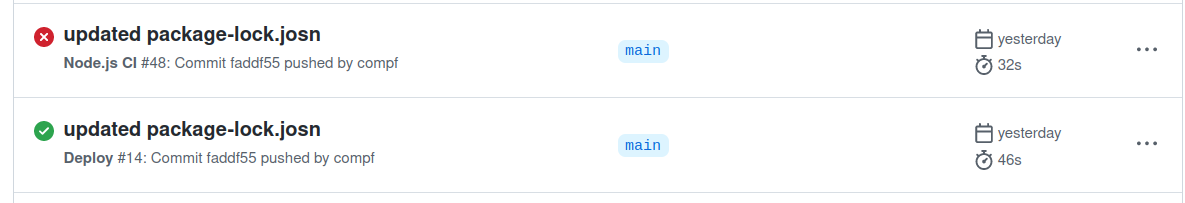
\includegraphics[width=\columnwidth]{figures/workflow_overview.png}
	    \caption{Übersicht über die ausgeführten Workflows}
	    \label{fig:workflow_overview}
	\end{figure}
	
	Durch einen Klick auf den Titel des Commits, wechselt Github auf eine weitere Seite, die grundsätzlich die gleichen Informationen wie zuvor enthält. Es ist jedoch hier möglich direkt zu der YAML-Datei zu gelangen, die diesen Workflow beschreibt. Ein weiterer Klick auf den Button mit dem Namen von dem definierten Jobs, wechselt auf eine weitere Seite, die die einzelnen Steps des Jobs auflistet und es ermöglicht, die Konsolenausgabe jedes Steps anzuzeigen. Auch eine Aufsplittung der Zeitdauer der einzelnen Steps wird angezeigt, sodass der Programmierer weiß, wie viel Zeit jeder Step benötigt. Abbildung \ref{fig:workflow_output} zeigt, wie eine solche Ausgabe auf der Konsole aussieht:
	\begin{figure}[h]
	    \centering
	    
	    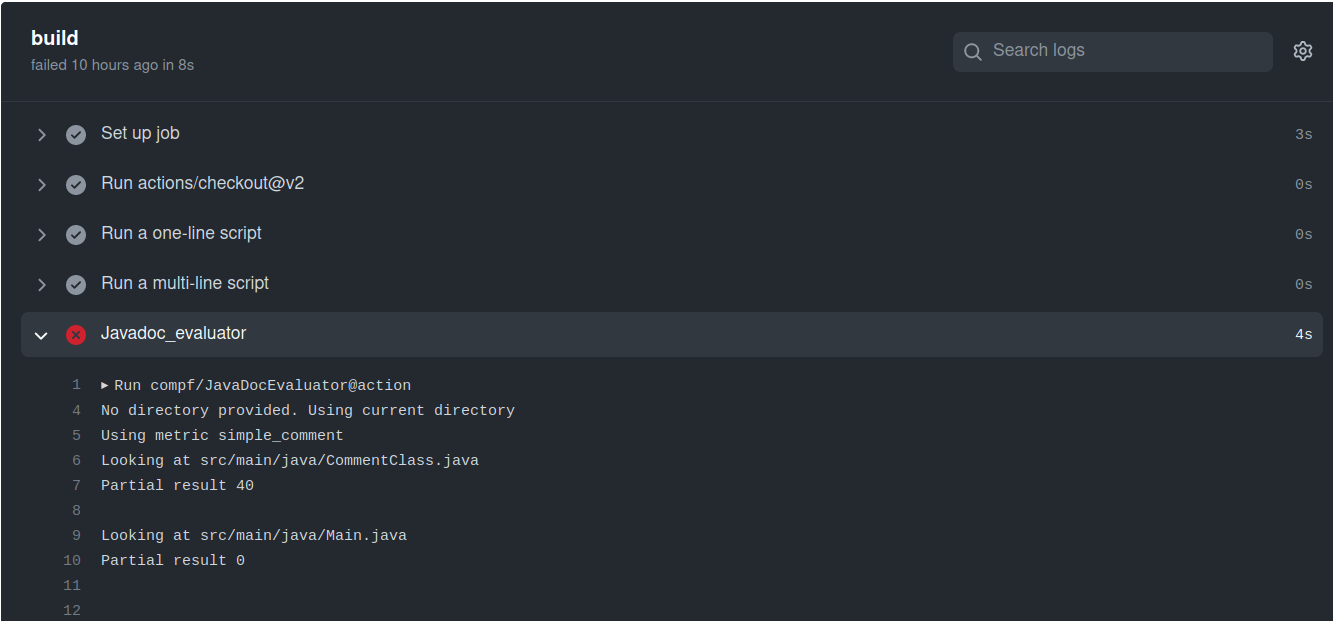
\includegraphics[width=\columnwidth]{figures/workflow_output.png}
	    \caption{Übersicht über die ausgeführten Workflows}
	    \label{fig:workflow_output}
	\end{figure}
\subsection{Erstellung einer eigenen Action}
Um eine eigene Github Action zu erstellen, muss in dem Hautpverzeichnis des Repositorys, in dem der Programmcode der Action liegt, eine Datei namens \enquote{action.yaml} oder \enquote{action.yml} erstellt werden. Abbildung \ref{lst:create_action_example} zeigt eine beispielshafte \enquote{action.yaml}
	\begin{figure}[h!]
			\lstinputlisting
			[caption={Beispielhafte Action-Konfigurationsdatei},
			label={lst:create_action_example},
			captionpos=b, basicstyle=\footnotesize, tabsize=1, showstringspaces=false,  numbers=left]
			{figures/create_action_example.yaml}
		\end{figure}
Zunächst wird der Name der Action und eine Beschreibung definiert. Anschließend können Eingabeparameter definiert werden, die später im Programm verwendet werden können. Zu jedem Parameter kann auch festgelegt werden, ob er zwingend erforderlich ist und den Standardwert des Parameters. Außerdem können Ausgabeparameter festgelegt werden, die spätere Actions als Eingabe nutzen können. Danach wird festgelegt, wie diese Action ausgeführt wird. Eine Action kann in einer Javascript-Umgebung, in einem einem Docker-Container, oder als Liste von verschiedenen Steps ausgeführt werden. Dies wird in den folgenden Unterabschnitten kurz beschrieben.
\subsubsection{Docker-Umgebung}
In einer Docker-Umgebung kann die Action ausgeführt werden, ohne dass der Nutzer der Action sich darüber Gedanken machen muss, welche Abhängigkeiten oder Voraussetzungen diese Action benötigt. Dies ermöglicht eine fehlertolerante Ausführung des Programmscodes. Das System kann dabei sehr frei konfiguriert werden. Allerdings laufen Actions in einer Docker-Umgebung langsamer als in einer Javascript-Umgebung. Außerdem kann zurzeit ein Action in einer Docker-Umgebung nur mittels eines Runners in Linux ausgeführt werden.

\subsubsection{Javascript-Umgebung}
Da viele GitHub Actions in Javascript programmiert werden, ist diese Umgebung als Option vorhanden. Es kann direkt eine geeignete Node-Umgebung installiert werden und eine Javascript-Datei mittels \textit{main} ausgeführt werden. 

\subsubsection{Composite-Action}
Eine sogenannte Composite-Action ermöglicht es mehrere Actions in eine Action zu vereinen und so wieder Code-Redundanz zu vermeiden. Die Syntax ist dabei ähnlich wie ein normaler Workflow. 

	
\section{General Background}
\label{sec:generalBackground} 

General background of the thesis. Most likely divided into several sections, which might might be in individual files.
	\section{Related Work}
\label{sec:relatedWork}

The related work of the literature related to your thesis.





\chapter{Main Part}
	

\chapter{Evaluation}
	\label{sec:evaluation}
	\newcommand{\checkpmd}{\textit{Checkstyle} und \textit{PMD} }
\newcommand{\doceval}{\textit{DocEvaluator} }
In diesem Kapitel soll das Programm evaluiert werden, um zu prüfen, ob das Programm (im Folgenden \textit{DocEvaluator}) eine gute heuristische Aussage über den Stand der Dokumentationsqualität treffen kann und in der Praxis auch einsetzbar ist. Dazu wird der \textit{DocEvaluator} mit \textit{Checkstyle} und \textit{PMD} verglichen, indem drei exemplarische Open-Source-Projekte mit allen drei Programmen analysiert werden und die Treffergenauigkeit und Geschwindigkeit der Programme verglichen werden. Zunächst müssen diese drei Projekte ausgewählt werden, was in Kapitel \ref{chapter:choosing_project} erläutert wird. Anschließend wird in Kapitel \ref{chapter:quality} beschrieben, wie die Evaluation der Treffergenauigkeit ermittelt wird. In Kapitel \ref{chapter:speed} wird die Geschwindigkeitsevaluation durchgeführt. Zum Abschluss der Evaluation werden die Ergebnisse der Evaluation in Kapitel \ref{chapter:eval_conclusion} resümiert. 

\section{Wahl der zu analysierenden Projekte}\label{chapter:choosing_project}
Zur Durchführung der Evaluation wurden verschiedene Softwareprojekte aus GitHub heruntergeladen. Grundsätzlich kann der Vergleich mit jedem Java-Projekt durchgeführt werden, dennoch wurden einige Bedingungen festgelegt, die bei der Auswahl der Projekte eine wichtige Rolle spielen. Diese Bedingungen werden in der folgenden Auflistung präsentiert:

\begin{enumerate}
    \item \label{enum:size} Die Projekte müssen mindestens einen Umfang von 10~000 \ac{LOC} haben
    \item \label{enum:already_cited} Die Projekte müssen bereits in einer in dieser Bachelorarbeit zitierten Quelle in puncto Dokumentationsqualität analysiert worden sein
    \item \label{enum:parsing_error}  Die Projekte sollen möglichst wenige Parsing-Fehler beim \doceval produzieren. Bei mehr als als zwei Fehlern wird ein Projekt nicht betrachtet. Können jedoch Fehler folgenlos behoben werden, so kann das Projekt dennoch betrachtet werden
    \item Das größte Projekt sollte mindestens zehnmal so groß sein wie das kleinste Projekt
\end{enumerate}

Die \ac{LOC} sollen nur als sehr grobe Heuristik der Größe eines Softwareprojektes verstanden werden und enthalten nur den reinen Code ohne Kommentare. Dabei wird heuristisch vermutet, dass mit steigender \ac{LOC} die Anzahl der Komponenten in einem Softwareprojekt steigt, wobei all diese Komponenten fehlerhaft (oder gar nicht) dokumentiert sein können. Somit dienen die \ac{LOC} als approximative Schätzung der zu erwartenden Fehler. 
 Durch die Bedingung in Nr. \ref{enum:size} wird sichergestellt, dass eine ausreichende Anzahl an Fehlern in der Dokumentation zu erwarten ist, um eine gute Analyse der Dokumentationsqualität  und eine aussagekräftige Bewertung der Geschwindigkeit zu ermöglichen. Durch die Bedingung in Nr.  \ref{enum:already_cited} werden nur Projekte in Betracht gezogen, die bereits in der wissenschaftlichen Literatur berücksichtigt wurden und daher (zumindest für den jeweiligen Autor der Quelle) geeignet für eine Analyse der Dokumentation sind. Mit der Bedingung in Nr. \ref{enum:parsing_error} wird eine Verzerrung zugunsten oder zuungunsten des \textit{DocEvaluators} vermieden, denn durch Parsing-Fehler können Komponenten falsch analysiert werden, die von den anderen Tools richtig analysiert werden. Indirekt wird dadurch gefordert, dass ein Projekt keine neueren Java-Funktionen verwendet, da  der \textit{DocEvaluator} nur Java bis Version 8 unterstützt. Die letzte Bedingung ist besonders für die Bewertung der Geschwindigkeit relevant, da so geprüft werden kann, ob der \doceval auch bei größeren Projekten noch in annehmbarer Zeit ein Ergebnis berechnen kann. 
 
 \subsubsection{Analysierte Projekte}\label{chapter:eval_projects}
 Die folgende Auflistung zeigt die gewählten Projekte für die Evaluation. In Klammern dahiner befinden sich die  (gerundeten) \ac{LOC}
 \begin{itemize}
  \item Log4J Version 1 (20~000)
    \item ArgoUML (17~000)
     \item Eclipse \ac{JDT} (400~000)
 \end{itemize}
 
 ArgoUML und Eclipse wurden in \cite[S.~74] {AutomaticQualityAssessmentofSourceCodeComments:TheJavadocMiner} bewertet, wobei hier nur Eclipse \ac{JDT} betrachtet werden soll, da das gesamte Eclipse-Projekt zu umfassend ist. Log4J wurde in \cite[S.~267] {@tComment:TestingJavadocCommentstoDetectComment-CodeInconsistencies} betrachtet. 

 Bei allen Projekten traten zunächst Parsing-Fehler auf. Dies lag allerdings in den meisten Fällen daran, dass auskommentierte Methoden noch einen Javadoc-Präfix hatten. Dies kann vom \doceval nicht korrekt verarbeitet werden. Da diese Methoden offensichtlich nicht verwendet werden und keinen Einfluss auf die Qualität der Dokumentation haben können, wurden sie ersatzlos entfernt. Bei einen Fehler in Eclipse \ac{JDT} konnte der \doceval eine Datei mit mehr als 3000 Codezeilen nicht verarbeiten. Diese Datei wurde bei der Evaluation von allen Programmen ignoriert.
\section{Analyse der Qualität}\label{chapter:quality}
Durch die Evaluation der Qualität soll geprüft werden, ob der \doceval trotz des in Kapitel \ref{chapter_conception}
 beschriebenen abstrakten Format eine Java-Datei richtig parsen kann und alle für die Dokumentation relevanten Informationen korrekt extrahieren kann. Zur Durchführung der Evaluation muss zunächst definiert werden, welche Funktionen der einzelnen Programme miteinander verglichen werden können, da die Programme unterschiedliche Aspekte der Dokumentation überprüfen und die Darstellung der Ergebnisse im Vergleich zum \textit{DocEvaluator} abweicht.

\checkpmd können als fehlersuchend bezeichnet werden. Sie prüfen die einzelnen Komponenten eines Programms und finden Abweichungen von vorher definierten Regeln. Eine solche Regel kann beispielsweise sein, dass jede öffentliche Methode dokumentiert sein muss, dass bestimmte Wörter nicht verwendet werden dürfen oder dass die Syntax der Dokumentation Fehler enthält. Damit sind sie vergleichbar mit den Metriken aus den Kapiteln \ref{chapter:metrics_coverage}  und \ref{chapter:metrics_errors}, welche ebenfalls bestimmte Fehler suchen und bei einem Verstoß gegen die Regeln eine Warnmeldung ausgeben. Allerdings berechnen \checkpmd keine Metriken, sondern finden nur die besagten Verstöße gegen die definierten Regeln. Somit kann ein Entwickler sehen, dasś ein Projekt beispielsweise 100 Verstöße gegen die Dokumentationsrichtlinien hat, erfährt aber nicht, ob die Anzahl der Verstöße unter Berücksichtigung der Projektgröße schwerwiegend ist und erhält keine normierte Bewertung, die dem Entwickler bei der Beurteilung der Dokumentationsqualität hilft. 

Im Gegensatz dazu verwendet der \doceval Metriken, die stets einen Wert von 0 bis 100 zurückgeben, sodass ein Entwickler weiß, dass ein hoher Wert für eine hohe Qualität steht. Außerdem kann der \doceval auch die Semantik des Kommentars heuristisch prüfen, um zu erfahren, ob der Kommentar verständlich ist und nicht redundant ist (vgl. Kapitel \ref{chapter:metrics_semantic}). Nichtsdestotrotz gibt der \doceval auch Warnmeldungen aus, wenn er bestimmte Komponenten schlechter bewerten muss.

Aus diesen Gründen wird die Evaluation nicht mit den Metriken an sich, sondern mit den Warnmeldungen der jeweiligen Tools durchgeführt. Jedes Programm wird mit einem Verweis auf das zu analysierende Projekt aufgerufen und die Ausgaben der Programme werden in separaten Dateien umgeleitet.  Diese Dateien dienen dann als Grundlage für die spätere Evaluation. 

\subsubsection{Durchführung der Evaluation}
Wie im vorherigen Absatz beschrieben, dienen die Logdateien der drei Programme als Datengrundlage für die Evaluation. Jede Zeile in diesen Logdateien enthält mindestens den Dateipfad des gefundenen Fehlers, die Zeilennummer des Fehlers und einen Fehlercode als Zeichenkette.  Wenn die drei Programme einen übereinstimmenden Fehler finden, sollte es in allen drei Logdateien einen Eintrag geben, bei dem der Dateipfad identisch ist, die Zeilennummer innerhalb eines gewissen Intervalls identisch ist und die der Fehlercode identisch ist. Die Zeilennummer muss nicht zwingen identisch sein, da  \checkpmd die exakte Zeile des Fehlers ausgeben, sodass beispielsweise bei einem unzulässigen Wort die exakte Zeile des Wortes genannt wird, während der \doceval nur die Zeile der betroffenen Komponente ausgibt. Da die drei Tools unterschiedliche Fehlercodes ausgeben, werden diese so kategorisiert, dass Verstöße, welche von mehr als einem Tool erkannt werden, einen eigenen Fehlercode erhalten. Alle anderen Verstöße erhalten einen allgemeinen programmspezifischen Fehlercode, der somit keine näheren Informationen über die Art des Fehlers hergibt.

Basierend auf diesen Vorbereitungen kann nun für jeden Fehler jedes Programm gefunden werden, das diesen Fehler gefunden kann. Beispielsweise kann ein Fehler von allen drei Programmen, nur von \textit{Checkstyle} oder nur von \textit{PMD} und \doceval gefunden werden. Mathematisch gesehen kann die Potenzmenge der Menge \textit{\{Checkstyle, PMD, DocEvaluator\}} genommen werden, wodurch alle möglichen Kombinationen an Programmen entstehen, die ein bestimmten Fehler erkennen können. Durch Zählen der Fehler pro Programmkombination lässt sich bewerten, welche Programme besonders viele Fehler finden, die andere Programme nicht erkennen und ob alle drei Programme viele identische Fehler finden. 


\subsubsection{Auswahl der Regeln}
Zum Vergleich der drei Programme müssen zunächst Regeln festgelegt werden, bei denen die Programme eine Warnmeldung ausgeben. Bei \checkpmd{} erfolgt die Konfiguration über  Extensible-Markup-Language-Dateien. Beim \doceval erfolgt die Konfiguration über das in Kapitel \ref{chapter:conf} beschriebene \ac{JSON}-Format. Bei der Auswahl der Regeln muss beachtet werden, dass \checkpmd auch andere Fehler wie z.~B. komplexe Methoden finden können. Diese sind in diesem Kontext nicht relevant und werden ignoriert. Außerdem können die drei Programme zum Teil unterschiedliche Fehler finden, da beispielsweise \textit{PMD} (anders als \textit{Checkstyle}) den Inhalt der Dokumentation auf das Auftauchen bestimmter Begriffe prüfen kann, \textit{Checkstyle} aber dafür (anders als \textit{PMD}) prüfen kann, ob die Block-Tags in der richtigen Reihenfolge definiert werden. Die letztere Regel wird vom \doceval in der ausgelieferten Fassung nicht geprüft. Alle drei Programme können jedoch prüfen, ob eine Komponente dokumentiert ist oder nicht. Tabelle \ref{tab:inters_rules} vergleicht die Überschneidungen der Regeln, welche die drei Programme anwenden können. Dabei stehen (sowohl hier als auch im Rest dieses Kapitels) die Abkürzungen \textit{CS} für \textit{Checkstyle} und \textit{DE} für \textit{DocEvaluator}.

\begin{table}[]
    \centering
    \begin{tabular}{m{4.5cm}|m{4.5cm}|m{4.5cm}}
     \textbf{CS} $\cap$ \textbf{DE}  & \textbf{PMD} $\cap$ \textbf{DE} & \textbf{PMD} $\cap$ \textbf{DE} $\cap$  \textbf{CS}  \\\hline
     \begin{itemize}
        \item Komponente dokumentiert
        \item Methode vollständig dokumentiert
         \item Fehler in Javadoc
     \end{itemize}
      & 
      \begin{itemize}
          \item  Komponente dokumentiert

          \item Bestimmte Wörter in Kommentar verbieten
      \end{itemize}
      & 
       \begin{itemize}
          \item  Komponente dokumentiert
         
      \end{itemize}
      \\\hline
    \end{tabular}
    \caption{Überschneidungen der Regeln der drei Programme}
    \label{tab:inters_rules}
\end{table}

Aus der Tabelle lässt sich entnehmen, dass der \doceval mit \textit{Checkstyle} die meisten Übereinstimmungen hat. Beide Programme können die Vollständigkeit der Methodendokumentation und typische Fehler in Javadoc-Kommentaren (wie z.~B. fehlerhaftes HTML) finden. PMD und der \doceval können bestimmte Wörter in der Dokumentation bemängeln, die in einer Dokumentation vermieden werden sollten. Alle drei Programme können das Vorhandensein der Dokumentation überprüfen. Allerdings ignoriert \textit{PMD} alle privaten Komponenten außer Felder. Vor allem bei Checkstyle gibt es zudem viele Regeln, die von den anderen beiden Programmen nicht gefunden werden und auf der Webseite \cite{checkstyle_doc_metrics} aufgelistet werden.

Da ein Vergleich der drei Tools somit nur eingeschränkt möglich ist, wird sich die qualitative Evaluation nur auf den Kernbereich beschränken. Es werden also nur die Regeln verwendet, die von mindestens zwei Tools unterstützt werden. Dies sind alle Regeln in Tabelle \ref{tab:inters_rules}. Da somit nur relativ leichte Fehler gefunden werden, können die Ergebnisse der Evaluation dazu verwendet werden, um die Parsing-Qualität zu ermitteln, denn wenn solche grundlegenden Fehler (wie z.~B. das Nichtvorhandensein der Dokumentation) nicht gefunden werden, besteht eine erhebliche Chance, dass eine Java-Datei falsch interpretiert wird. 



\subsection{Ergebnisse}

Tabelle \ref{tab:eval_results} listet die Anzahl der gefundenen Fehler (gemäß Tabelle \ref{tab:inters_rules}) auf. In den Spalten werden die die Fehler nach dem Projekt gruppiert. Die ersten drei Zeilen beschreiben, wie viele Fehler die einzelnen Tools pro Projekt gefunden haben. So hat  der \textit{DocEvaluator} 1710 Fehler in \textit{Log4J} gefunden.  In den übrigen Zeilen wird aufgeführt, welche Kombinationen der Tools wie viele Fehler gefunden haben. Die Zeile mit der ersten Spalte \enquote{\{PMD, DE\}} beschreibt beispielsweise, dass \textit{PMD} und der  \textit{DocEvaluator} 41 Fehler bei \textit{Log4J}, 264 Fehler bei \textit{ArgoUML} und 253 Fehler bei \textit{Eclipse \ac{JDT}} gefunden haben. Diese Fehler wurden nicht von \textit{Checkstyle} gefunden.  
\begin{table}[]
    \centering
\begin{tabular}{c|c|c|c}
          & Log4J & ArgoUML & Eclipse \ac{JDT} \\ \hline
|DE|            & 1~710 & 10~054  & 17~380      \\ \hline
|CS|            & 1~590 & 9~961   & 17~638      \\ \hline
|PMD|           & 1~008 & 9~051   & 12~702      \\ \hline\hline
\{DE\}          & 108   & 124     & 555         \\ \hline
\{CS\}          & 26    & 285     & 273         \\ \hline
\{PMD\}         & 86    & 377     & 298         \\ \hline
\{PMD, DE\}     & 41    & 264     & 253         \\ \hline
\{CS, DE\}      & 683   & 1~266    & 5~214       \\ \hline
\{PMD, CS\}     & 3     & 10      & 793         \\ \hline
\{PMD, CS, DE\} & 878   & 8~400   & 11~358      \\ \hline
\end{tabular}
    \caption{Anzahl der Fehler pro Projekt}
    \label{tab:eval_results}
\end{table}

Aus der Tabelle ist ersichtlich, dass die stets über 50~\% aller Fehler von allen drei Tools gefunden werden. Bei \textit{Eclipse \ac{JDT}} und \textit{Log4J} werden mehr als ein Viertel der Fehler von der Kombination  \textit{DocEvaluator} und \textit{Checkstyle} gefunden. Beim Projekt \enquote{ArgoUML} liegt diese Quote bei weniger als 15~\%.  Weniger als 10~\% der Fehler werden nur von einem Tool erkannt. 

Die Überschneidungen der Fehler lassen sich auch mit Venn-Diagrammen darstellen.  Die Abbildungen \ref{fig:log4j_venn}, \ref{fig:argo_venn} und  \ref{fig:eclipse_venn} zeigen für jedes Projekt die Überschneidungen der gefundenen Fehler. Die Abbildung \ref{fig:legend_venn} ist die Legende dieser drei Abbildungen:


\begin{figure}[ht!]

   \begin{subfigure}[b]{0.4\textwidth}
    \centering
\includesvg[scale=0.7,width=\textwidth]{figures/chapter5/log4j.svg}
    \caption{Venn-Diagramm: Log4J}
    \label{fig:log4j_venn}
\end{subfigure}
\hfill
\begin{subfigure}[b]{0.4\textwidth}
    \centering
\includesvg[scale=0.7,width=\textwidth]{figures/chapter5/argo.svg}
    \caption{Venn-Diagramm: ArgoUML}
    \label{fig:argo_venn}
\end{subfigure}
\hspace{10cm}
\begin{subfigure}[b]{0.4\textwidth}
    \centering
\includesvg[scale=0.7,width=\textwidth]{figures/chapter5/eclipse.svg}
    \caption{Venn-Diagramm: Eclipse \ac{JDT}}
    \label{fig:eclipse_venn}
\end{subfigure}
\hspace{3.4cm}
\begin{subfigure}[b]{0.25\textwidth}
    \centering
\includesvg[width=1\textwidth]{figures/chapter5/legende_venn.svg}
\vspace{0.3cm}
    \caption{Legende der Venn-Diagramme}
    \label{fig:legend_venn}
\end{subfigure}
\end{figure}

  Auch hier zeigt der graue Bereich visuell, dass die drei verglichenen Tools viele Fehler gemeinsam finden . Dies ist vor allem bei \textit{ArgoUML} deutlich, da der graue Kreis fast alle anderen Kreise großflächig überdeckt. Bei den anderen beiden Projekten ist zudem eine große Überschneidung von \textit{Checkstyle} und \doceval (hellbraun) zu erkennen. Bei\textit{Log4J} zeigt das Diagramm einen im Vergleich zu den anderen Projekten größeren Bereich (dunkelblau) an Fehlern, die nur von \textit{PMD} gefunden werden. Auch der Bereich der exklusiv vom \textit{DocEvaluator} gefundenen Fehler (rot) ist bei \textit{Log4J} größer. Die nur vom \textit{DocEvaluator} und \textit{PMD} gefundenen Fehler (lila) sind bei  \textit{Eclipse \ac{JDT}} nicht zu erkennen, bei den anderen Venn-Diagrammen allerdings schon. Dafür scheint es bei  \textit{Eclipse \ac{JDT}} relativ viele Fehler zu geben, die nur von \checkpmd gefunden werden, da der hellblaue Abschnitt nur dort sichtbar ist. Außerdem gibt es bei  \textit{Eclipse \ac{JDT}} mehr Fehler, die nur von \textit{Checkstyle} gefunden werden, da der grüne Bereich größer ist. 

Um die Trefferrate mathematisch auszudrücken, kann die Formel
\begin{equation}\label{eq1}
    1-\frac{\text{\{DE\}}}{|\text{DE}|}
\end{equation} verwendet werden. Diese gibt in Prozent an, wie viele Fehler, die vom \doceval gefunden werden, auch von den anderen beiden Tools gefunden werden. Demgegenüber kann auch ermittelt werden, wie viele Fehler von \textit{Checkstyle} oder \textit{PMD} gefunden wurden, die auch vom \doceval erkannt wurden:

\begin{equation}\label{eq2}
    1-\frac{\text{\{CS\}}+\text{\{PMD\}}+\text{\{CS,PMD\}}}{|\text{PMD}|+|\text{CS}|}
\end{equation}

Tabelle \ref{tab:hit_rate} zeigt basierend auf den genannten Formeln (\ref{eq1} und \ref{eq2}) die Treffergenauigkeit des \textit{DocEvaluators} für jedes analysierte Projekt:
\begin{table}[]
    \centering
    \begin{tabular}{c|c|c|c}
    Formel & Log4J & ArgoUML & Eclipse \ac{JDT} \\ \hline
    \ref{eq1} &   93.68~\% &	98.77~\% &	96.81~\% \\\hline
     \ref{eq2} & 95.57~\% &	96.47~\% &	95.50~\% \\\hline

    \end{tabular}
    \caption{Trefferrate des \textit{DocEvaluators} gemäß den Formeln \ref{eq1} und \ref{eq2}}
    \label{tab:hit_rate}
\end{table}
Es ist klar erkennbar, dass die Trefferrate unabhängig von der Formel und den analysierten Projekt größer als 90~\% ist, sodass die meisten Fehler, die vom \doceval gefunden werden, von mindestens einem anderen Tool gefunden werden und die meisten Fehler, die von \textit{Checkstyle} oder \textit{PMD} gefunden werden, auch vom \doceval gefunden werden.






\subsection{Bewertung der Qualitätsevaluation}
Insgesamt zeigt die Evaluation der Qualität, dass der \doceval eine hohe Abdeckung mit \checkpmd hat und somit die meisten von diesen Tools gefundenen Fehler auch findet. Somit ist das abstrakte Format zur Repräsentation einer Quellcodedatei geeignet, um die meisten Aspekte, welche für die Dokumentation relevant sind, zu beschreiben. Allerdings wurde diese Evaluation auf größere Projekte (über 10~000\ac{LOC}) beschränkt, sodass nicht geprüft wurde, ob der \doceval auch bei kleineren Projekten eine genaue Einschätzung der Dokumentationsqualität gibt. Tendenziell wird die Trefferrate kleiner sein, da durch die geringere Größe jeder nicht gefundene Fehler ein höheres Gewicht hat. 

Während der Evaluation wurde geprüft, warum einige Fehler nicht vom \doceval gefunden wurden. In einigen Fällen waren dies einfache Fehler, die bereits behoben wurden, sodass dadurch die Trefferrate erhöht wurde. In anderen Fällen gibt es größere strukturelle Probleme, die nicht mehr leicht behebbar sind. Einige dieser Fehler werden im Folgenden präsentiert: 
\subsubsection{Fehler durch verschiedene Zeilennummerierung}

Einige Fehler sind keine Fehler des \textit{DocEvaluators} an sich, sondern sind in der Methodik der Evaluation begründet. Um gemeinsame Fehler zu finden, müssen die gefundene Fehler pro Tool abgeglichen werden, wozu die Zeilennummer elementar ist. Allerdings gibt es Unterschiede bei der Festlegung der Zeilennummer. Der \doceval verwendet in seiner Logausgabe einen Zeilennummerintervall, der mit Zeile des Bezeichners der Komponente endet und dessen Anfang durch Subtraktion der Anzahl der Zeilen des Dokumentation von der Zeile des Bezeichners definiert wird. Die anderen Tools verwenden die exakte Zeile eines Fehlers. In den meisten Fällen ist dies kein Problem, da diese Zeilennummer von \checkpmd innerhalb des vom \doceval beschriebenen Intervalls liegen muss. Listing \ref{lst:multiline_method} zeigt ein Beispiel, wo es problematisch wird.

		\begin{figure}[ht!]
			\lstinputlisting
			[caption={Methode auf viele Zeilen verteilt},
			label={lst:multiline_method},
			captionpos=b,language=java, basicstyle=\footnotesize, tabsize=1, showstringspaces=false,  numbers=left]
			{figures/chapter5/multiline_method.java}
		\end{figure}
Besonders an dieser Methode ist, dass die Parameter auf verschiedenen Zeilen verteilt ist. Während \textit{Checkstyle} bei einem undokumentierten Parameter die exakte Zeile eines nicht dokumentierten Parameters ausgibt (z.~B. Z. 5), würde der \doceval die Zeilen 1 bis 4 ausgeben, da die Dokumentation bei Zeile 1 beginnt und der Bezeichner der Komponente in Zeile 4 definiert ist. Ähnlich problematisch ist es, wenn zwischen der Dokumentation und dem Bezeichner noch Annotationen stehen, sodass der Bezeichner um eine Zeile nach unten rutscht.  

\subsubsection{Klassen in Methoden}

In Java können Klassen in Methoden deklariert werden bzw. anonyme Klassen direkt instantiiert werden. Diese Klassen können ebenfalls Javadoc besitzen, werden allerdings vom \doceval ignoriert, da der \doceval jeglichen Code in Methoden nur unstrukturiert als Zeichenkette speichert und nicht weiterverarbeitet. Die anderen beiden Tools prüfen auch diese Klasse, sodass sie entsprechend einige Fehler finden, die der \doceval nicht mehr finden kann. 


\subsubsection{Fehler in einzeiligen Kommentaren bei PMD}
Anders als der\doceval und \textit{Checkstyle} berücksichtigt \textit{PMD} auch einzeilige Kommentare. Wenn ein einzeiliger Kommentgar ein unzulässiges Wort enthält, so würde \textit{PMD} einen Fehler melden, aber der \doceval nicht, da er nur Javadoc-Kommentare prüft. Dadurch kommt es zu einer Verzerrung und der Anteil der alleinig von \textit{PMD} gefundenen Fehler wird überschätzt.  


\clearpage

 \section{Analyse der Geschwindigkeit} \label{chapter:speed}
 In diesem Abschnitt wird der \doceval mit \checkpmd in Bezug auf die Geschwindigkeit verglichen. Damit soll geprüft werden, ob das Tool neben einer guten Qualität auch in einer angemessenen Zeit ein Ergebnis liefert. Dies ist im \ac{CI/CD}-Kontext wichtig, da bei einer langen Laufzeit des Tools  die Bereitstellung eines geprüften Softwareprojektes verzögert wird und somit die Produktivität reduziert wird. 
 
 \subsubsection{Durchführung der Geschwindigkeitsevaluation}
 Zur Durchführung der Evaluation der Geschwindigkeit analysieren die drei Tools die in Kapitel \ref{chapter:eval_projects} Projekte. Damit jedes Programm fair behandelt wird und eine ungefähr gleiche Menge an Analysen durchführen kann, werden die Regeln so beschränkt, dass nur noch das Vorhandensein von Dokumentation geprüft wird. So wird verhindert, dass beispielsweise der \textit{DocEvaluator} und \textit{Checkstyle} die Dokumentation von Methodenparameter überprüfen, während \textit{PMD} dies ignoriert. Bei jeder Analyse wird die Zeit gemessen, die vom Start eines Tools bis zu dessen Beendigung vergehen. 
 
 Die Ausgabe jedes Tools wird auf \enquote{dev/null} umgeleitet, sodass jegliche Ausgabe ignoriert wird. Dadurch können Schwankungen unberücksichtigt bleiben, die bei der Verwendung von Eingabe- und Ausgabegeräten auftreten, damit die Ergebnisse näher an der tatsächlichen Verarbeitungsgeschwindigkeit sind.  Nachteilhaft an diesem Vorgehen ist, dass die Tools im Praxiseinsatz eine Ausgabe produzieren müssen, um überhaupt den Entwickler helfen zu können, sodass dieser wichtige Aspekt hier ignoriert wird. 
 
 Die Analyse jedes Projektes mit jedem Tool wird zehnmal durchgeführt, um Schwankungen durch Hintergrundprozesse oder andere Einflussfaktoren auszugleichen. Die Evaluation der Geschwindigkeit wird auf einem Laptop mit dem Prozessor \enquote{i7-1165G7} mit 16 GB Arbeitsspeicher durchgeführt. Dabei wurden alle Programme auf dem Computer geschlossen und die Berechnungen wurden ohne grafische Benutzeroberfläche durchgeführt, um die Schwankungen der Laufzeit zu minimieren.  
 \subsection{Ergebnisse}\label{chapter:eval_speed_result}
 Die Tabellen \ref{tab:median_speed} und \ref{tab:std_speed} zeigen den Median und die Standardabweichung der benötigten Durchlaufzeit pro Tool und Projekt in Sekunden. Die Rohdaten, also alle zehn Durchlaufszeiten pro Tool und Projekt, sind im Anhang \ref{chapter:raw_speed_data} zu finden. Die Abbildungen \ref{fig:log4j_box}, \ref{fig:argo_box} und \ref{fig:eclipse_box} visualisieren den Inhalt der Tabellen als Boxplot. Diese Abbildungen sind ebenfalls im Anhang \ref{appendix:boxplots} in maximaler Größe dargestellt: 
 \begin{table}[ht!]
     \centering
     \begin{tabular}{c|c|c|c}
        & DE & CS & PMD  \\\hline
        Log4J & 2.538 & 2.30 & 1.907\\\hline 
        ArgoUML & 16.965 & 9.301 & 7.917 \\\hline
        Eclipse \ac{JDT} & 69.148 & 27.316 & 21.586
     \end{tabular}
     \caption{Median der Performance in Sekunden}
     \label{tab:median_speed}
 \end{table}
 
  \begin{table}[ht!]
     \centering
     \begin{tabular}{c|c|c|c}
        & DE & CS & PMD  \\\hline
        Log4J & 0.077 &  0.174 &  0.068\\\hline 
        ArgoUML & 0.197 &  0.083 & 0.157 \\\hline
        Eclipse \ac{JDT} & 1.594 & 0.265 & 0.270\\\hline
     \end{tabular}
     \caption{Standardabweichung der Performance in Sekunden}
     \label{tab:std_speed}
 \end{table}
 
 \begin{figure}
    \begin{subfigure}[b]{0.5\textwidth}
    \centering
\includesvg[width=\textwidth]{figures/chapter5/log4j_speed_boxplot.svg}
    \caption{Boxplot: Log4J}
    \label{fig:log4j_box}
\end{subfigure}
\hspace{0.1cm}
 \begin{subfigure}[b]{0.5\textwidth}
    \centering
\includesvg[width=\textwidth]{figures/chapter5/argo_speed_boxplot.svg}
    \caption{Boxplot: ArgoUML}
    \label{fig:argo_box}
\end{subfigure}

 \begin{subfigure}[b]{0.7\textwidth}
    \centering
\includesvg[,width=\textwidth]{figures/chapter5/eclipse_speed_boxplot.svg}
    \caption{Boxplot: Eclipse \ac{JDT} }
    \label{fig:eclipse_box}
\end{subfigure}
   
 \end{figure}
 

Aus den Tabellen und Boxplot-Diagrammen wird ersichtlich, dass der \doceval im Durchschnitt länger benötigt, um die Projekte zu bewerten. Wie aus dem Boxplot-Diagramm \ref{fig:log4j_box} zu entnehmen ist, gab es nur bei Log4J einen Ausreißer, bei dem \textit{Checkstyle} mehr Zeit benötigt hat.   Ansonsten war \textit{Checkstyle} stets schneller als der \textit{DocEvaluator} \textit{PMD} analysiert am schnellsten ein Projekt. Der Unterschied in der Laufzeit zwischen dem \doceval und den anderen Tools steigt stark  mit wachsender Größe des analysierten Projektes.  Bei dem kleinsten Projekt \textit{Log4J} benötigt der \doceval  durchschnittlich die 1.103-fache Zeit im Vergleich zu \textit{Checkstyle}. Bei dem größten Projekt \textit{Eclipse \ac{JDT}} benötigt der \doceval durchschnittlich 2.53-mal so viel Zeit wie \textit{Checkstyle}. Beim \doceval und \textit{PMD} steigt die Standardabweichung mit der Größe des Projektes, während dieser Trend bei \textit{Checkstyle} nicht so eindeutig ist.

Bei dem Boxplot-Diagramm \ref{fig:log4j_box} zu \textit{Log4J} ist auch erkennbar, dass Ausreißer der Laufzeit nach oben häufiger sind als nach unten, da der Median sich stets im unteren Bereich des Boxplot-Quartile befindet. Bei den anderen Projekten ist dies aufgrund des größeren Zeitabstand  zwischen dem \doceval und den anderen Tools  und der daraus resultierenden Verkleinerung der einzelnen Boxplots  nicht so klar im Boxplot ersichtlich, allerdings stimmt diese Aussage größtenteils auch dort. Nur bei der Analyse von \textit{ArgoUML} durch den \doceval (Abbildung \ref{fig:argo_box}) scheinen Abweichungen nach unten häufiger zu sein.

\subsection{Bewertung der Ergebnisse}
Insgesamt zeigt die Evaluation der Geschwindigkeit, dass der \doceval langsamer arbeitet als die anderen Programmen. Allerdings  bleibt die Laufzeit auf einen angemessenen Niveau, da die Verarbeitung von dem größten Projekt \enquote{Eclipse \ac{JDT}} mit 400.000 \ac{LOC} im Durchschnitt nur etwas mehr als einer Minute benötigt. Nichtsdestotrotz ignoriert diese Analyse, dass die Ausgabe von Ergebnissen über die Konsole hier nicht berücksichtigt wurde und nur eine einfache Metrik angewendet wurde. Bei einem Experiment mit aktivierter Ausgabe wurden ähnliche Ergebnisse produziert, insbesondere ist der \doceval weiterhin das langsamste Programm. 

Für die schlechtere Laufzeit des \doceval im Vergleich zu \checkpmd lassen sich zwei Hauptargumente finden. So soll \textit{Node.Js}, welches die Plattform des Tools ist, langsamer sein als Java, in dem \checkpmd programmiert sind \cite{node_java_speed}.  Außerdem ist zu beachten, dass der \doceval Metriken berechnen soll und daher die Zwischenergebnisse aller Komponenten speichern muss, um daraus ein Gesamtergebnis mittels eines arithmetischen Mittelwerts oder eines anderen Algorithmus' berechnen zu können. Auch wenn dieses Gesamtergebnis bei der Laufzeitevaluation uninteressant ist, wird es dennoch berechnet, was zusätzliche Laufzeit benötigt. Dies erklärt auch die starke Steigerung des Zeitaufwands mit größeren Projekten.

\section{Fazit der Evaluation}\label{chapter:eval_conclusion}

Insgesamt zeigt die Evaluation sowohl bezüglich der Qualität als auch der Geschwindigkeit, dass der \doceval mit den anderen Tools mithalten kann. Zwar wird nicht jeder Fehler gefunden, aber die Trefferrate ist hoch und durch die Verwendung eines abstrakten Formates, das für mehrere Programmiersprachen geeignet ist, sind solche Abstriche nicht vermeidbar. 

Auch bei der Geschwindigkeit zeigt sich, dass der \doceval zwar im Extremfall zweieinhalbmal langsamer ist als die anderen Tools, allerdings ist die Laufzeit mit knapp 70 Sekunden im Extremfalls bei einem großen Projekt noch in einem (relativ) angemessenen Rahmen. Nichtsdestotrotz ist es eine Überlegung wert, genauere Analysen durchzuführen, um die Geschwindigkeit des \textit{DocEvaluators} verbessern zu können. 

\chapter{Conclusion and Future Work}
\label{sec:conclusion}
In diesem Kapitel wird ein Ausblick gegeben und ein Fazit gezogen. Dazu wird erläutert, wie das Tool ergänzt werden kann und welche Probleme bei einer Erweiterung auftreten können
\section{Erweiterung des Tools}
Es gibt viele Ideen, um weitere Funktionen für den \textit{DocEvaluator} zu implementieren, dies es wegen der begrenzten Bearbeitungszeitraums allerdings nicht in der Abgabeversion geschafft haben. Diese Vorschläge und Ideen werden nachfolgend erläutert.
\subsubsection{Weitere Programmiersprachen}
In der ausgelieferten Version unterstützt das Tool nur Java, es wurde aber prinzipiell so konzipiert, dass eine Erweiterung auf weitere Programmiersprachen möglich ist. Dazu muss eine geeignete Parser-Klasse geschrieben werden, die eine Quellcodedatei in das in Kapitel \ref{chapter_conception} beschriebene Format überführt. 

Da sich die Programmiersprachen in einigen Punkten besondere Funktionen haben, müssen diese geeignet abstrahiert werden. Beispielsweise müssen Eigenschaften in C\# in einer geeigneten Unterklasse von \textit{Component} dargestellt werden. Dazu kann eine neue abgeleitete Klasse erstellt werden. Alternativ kann die Klasse \textit{SingleMemberComponent}  benutzt werden, da sich eine C\#-Eigenschaft von der Benutzung sich kaum von einem gewöhnlichen Feld unterscheidet.

Außerdem muss dann für die Programmiersprache die sprachspezifischen Hilfsmethoden passend überschrieben werden.

\subsubsection{Unterstützung mehrere Programmiersprachen}
Eine weitere Idee ist es, mehrere Programmiersprachen zu unterstützt, sodass  beispielsweise die Dokumentationsqualität von einen gemixten Java- und Python-Projekt bewertet werden kann. Dazu kann je nach Dateiendung ein passender Parser aufgerufen werden und dann die sprachunabhängigen Metriken angewendet werden.

\subsubsection{Unterstützung weitere natürlicher Sprachen}
In der ausgelieferten Fassung unterstützt das Tool nur Englisch als Sprache. Beispielsweise sind alle \ac{NLP}-Metriken sehr auf die englische Sprache bezogen. Eine Erweiterung auf andere Sprachen könnte in Erwägung gezogen werden. 

\subsubsection{Unterstützung von anderen CI/CD-Plattformen}
Neben GitHub bietet auch GitLab eine Plattform zur automatisierten Ausführung von Programmcode bei bestimmten Ereignissen an. Da GitHub nicht die einzige Plattform zum Arbeiten mit Softwareprojekten ist, wäre eine Erweiterung auf andere Plattformen sinnvoll. Dabei könnte auch eine Abstrahierung geprüft werden, um eine Portierung auf andere \ac{CI/CD}-Plattformen so einfach wie möglich zu machen. 









%Prints references
\printbibliography

%\ac{Abk.}         % fügt die Abkürzung ein, außer beim ersten Aufruf, hier wird die Erklärung mit angefügt
%\acs{Abk.}        % fügt die Abkürzung ein
%\acf{Abk.}        % fügt die Abkürzung UND die Erklärung ein
%\acl{Abk.}        % fügt nur die Erklärung ein

%\chapter*{Acronyms}
\addchap{Acronyms}

%%%%%%%%%%%%%%%%%%%%%%%
\begin{acronym}[E/E/PE] %sorgt fuer proper indention
	\acro{ATL}{\emph{Atlas Transformation Language}}
	\acro{BMWi}{\emph{Bundesministerium für Wirtschaft und Energie}}
	\acro{CIM}{\emph{Computation-Independent Model}}
	\acro{CDC}{\emph{Code-level design choice}}
	\acro{CR}{\emph{Code-level requirement}}
	\acro{CI/CD}{Continuous Integration/Continuous Delivery}
	\acro{CRC}{\emph{Cycling Redundancy Checks}}
	\acro{E/E/PE}{\emph{Electrical/Electronic/Programmable Electronic}}
	\acro{ECC}{\emph{Error Detecting and Correcting Codes}} 
	\acro{EMF}{\emph{Eclipse Modeling Framework}}
	\acro{EGL}{\emph{Epsilon Generation Language}}
	\acro{EOL}{\emph{Epsilon Object Language}}
	\acro{Epsilon}{\emph{Extensible Platform of Integrated Languages for mOdel maNagement}}
	\acro{FS}{\emph{Functional Safety}}
	\acro{HAL}{\emph{Hardware Abstraction Layer}}
	\acro{HolMES}{\emph{Holistische Modell-getriebene Entwicklung für Eingebettete Systeme unter Berücksichtigung unterschiedlicher Hardware-Architekturen}}
	\acro{IDE}{\emph{Integrated Development Environment}}
	\acro{JVM}{\emph{Java Virtual Machine}}
	\acro{LOC}{\emph{Lines of Code}}
	\acro{MISRA}{\emph{Motor Industry Software Reliability Association}}
	\acro{MBU}{\emph{Multi Bit Upset}}
	\acro{MDA}{\emph{Model Driven Architecture}}
	\acro{MDC}{\emph{Model-level design choice}}
	\acro{MDD}{\emph{Model Driven Development}}
	\acro{MDE}{\emph{Model Driven Engineering}}
	\acro{MOF}{\emph{Meta Object Facility}}
	\acro{MR}{\emph{Model-level requirement}}
	\acro{NLP}{\emph{Natural Language Processing}}
	\acro{OCL}{\emph{Object Constraint Language}}
	\acro{OMG}{\emph{Object Management Group}}
	\acro{PIM}{\emph{Platform-Independent Model}}
	\acro{PSM}{\emph{Platform-Specific Model}}
	\acro{SER}{\emph{Soft Error Rate}}
	\acro{SEU}{\emph{Single Event Upset}}
	\acro{TMR}{\emph{Triple Modular Redundancy}}
	\acro{UML}{\emph{Unified Modeling Language}}
	


%\acro{cMOF}{\emph{complete MOF}}
%\acro{eMOF}{\emph{essential MOF}}

%	\acro{ETL}{\emph{Epsilon Transformation Language}}
%	\acro{EWL}{\emph{Epsilon Wizard Language}}

	
\end{acronym} %See inside for usage of acronmys
\clearpage 

%Appendix (comes after bibliography)

\renewcommand\appendixpagename{Anhänge}
\begin{appendices}


\chapter{Änderungen an der Parserdatei}\label{chapter:appendix_parser_changes}

\begin{table}[h!]
    \centering
    \begin{tabular}{m{0.75cm}|m{4cm}|m{10cm}}
        \textbf{Zeile} & \textbf{Änderung} & \textbf{Begründung} \\
         \hline
        116 & Deklaration Kommentar & Hier wird ein mehrzeiliger Kommentar definiert, dies ist hier ein Alias für den Token \textit{JCOMMENT}\\
        \hline
        127--128 & \textit{comment} als mögliches Präfix in Klassenmember & Hier wird dem Parser mitgeteilt, dass ein Bestandteil einer Klasse wie z. B. eine Methode einen Javadoc-Kommentar besitzen kann\\
        \hline
        47 & \textit{comment} als mögliches Präfix vor Datentyp & Hier wird dem Parser mitgeteilt, dass ein Datentyp (Klasse, Schnittstelle etc. ) einen Javadoc-Kommentar haben kann \\
        \hline
        404 & Zulassung von Javadoc in Methoden & Da Javadoc-Kommentare an beliebigen Stellen auftauchen können, auch wenn es nicht empfohlen wird und keinen Mehrwert bietet, wird hier sichergestellt, dass solche Kommentare nicht zu Warnungen oder Fehler von ANTLR4 führen. Diese Javadoc-Kommentare werden nichtsdestotrotz später ignoriert\\
        \hline
        34, 38& Zulassung von Kommentaren vor Paketdeklarationen und Imports & Hier werden Kommentare auch vor Paketdeklarationen und Import-Statements erlaubt, was vor allem bei Klassen mit Urheberrechtsangabe sinnvoll ist\\
        \hline
        105 & Zulassung von Kommentaren bei Enumerationen & Zwar werden Javadoc-Kommentare in Enumerationen mit diesem Tool nicht betrachtet, sie führen aber dennoch zu Warnungen und Fehlermeldungen. Daher werden sie hier zugelassen, aber später ignoriert \\
        \hline
        82, 83 & Erzeugung eines separaten Knotens für \textit{Extends}- und \textit{Implements}-Deklarationen & In der originalen Version der Parserdatei wurde die Definition der Basisklasse bzw. der implementierten Schnittstellen direkt über die Tokens \textit{EXTENDS} bzw. \textit{IMPLEMENTS} gelöst. Dies wurde in einem neuen Knoten \textit{extendClass} bzw. \textit{implementInterfaces} ausgegliedert, um so das Parsing etwas zu vereinfachen  \\
         
    \end{tabular}
    \caption{Änderungen an der Parserdatei}
    \label{tab:parser_changes}
\end{table}

\chapter{UML-Diagramm: Parser}\label{appendix_parsing_uml}
\begin{figure}[ht!]
\fontsize{5}{10}\selectfont
    \centering
    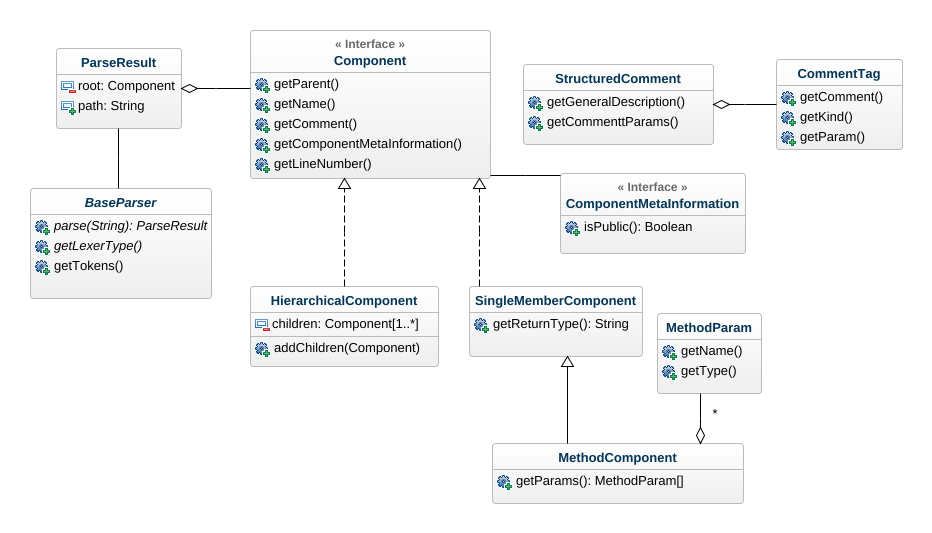
\includegraphics[height=9cm,keepaspectratio,angle=90]{figures/uml/parsing.png}
    \caption{UML-Diagramme aller Klassen, die relevant für das Parsen sind}
    \label{fig:uml_parsing}
\end{figure}
\chapter{UML-Diagramm: Metriken}\label{appendix_metrics_uml}
\begin{figure}[ht!]
\fontsize{5}{10}\selectfont
    \centering
    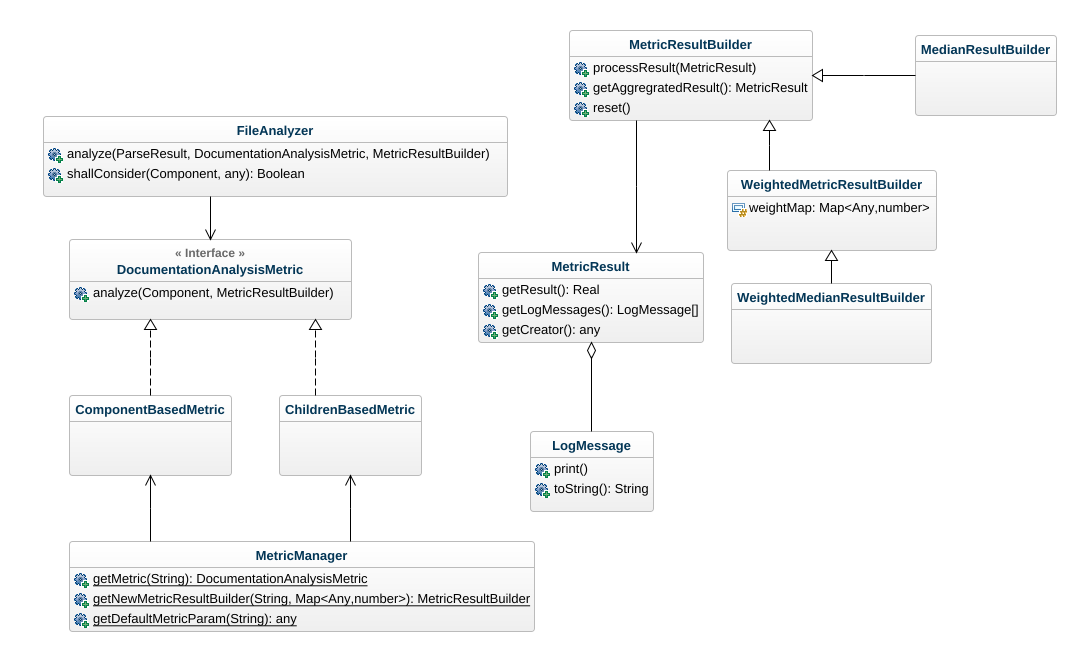
\includegraphics[height=10cm,keepaspectratio,angle=90]{figures/uml/metriken.png}
    \caption{UML-Diagramme aller Klassen, die relevant für die Metriken sind}
    \label{fig:uml_metrics}
\end{figure}
\chapter{Konfiguration des Tools}
\begin{description}
        \item[include]  Alle Dateien, die bei der Bewertung der Dokumentationsqualität berücksichtigt werden müssen
        \item[Exclude]  Teilmenge von include, enthält Dateien, die nicht weiter betrachtet werden müssen
        \item[metrics]  Alle Metriken, die das Tool verwenden soll. Dies ist ein Array von Objekten mit der Struktur \enquote{(name,weight, unique\_name, params)}, wobei \textit{weight} das Gewicht der jeweiligen Metrik ist (Bei Algorithmen ohne Relevanz des Gewichts wird es ignoriert), \textit{name} der Name der Metrik und \textit{params} ein Objekt mit den Parametern der Metrik
        \item[absolute\_threshold] Mindestwert der Bewertung, die erreicht werden muss, sonst wird die Dokumentationsqualität nicht akzeptiert
       
          \item[builder] Der Algorithmus/\textit{ResultBuilder}, der die einzelnen Ergebnisse verarbeitet.
        
        \item[parser]  Kann verwendet, um die zu parsende Programmiersprache zu wählen. Dazu muss \textit{ParserFactory} angepasst werden
        
        \item[path\_weights] Ein Array von Objekten der Struktur \enquote{(path,weight)}. Wird verwendet, um einzelne Pfade höher oder niedriger zu gewichtet
        
         \item[component\_weights] Ein Array von Objekten der Struktur \enquote{(name,weight)}. Wird verwendet, um einzelne Komponenten höher oder niedriger zu gewichtet
         
         \item[default\_path\_weight] Das Standardgewicht für eine Datei, wenn keine passende Gewichtung gefunden wurde
         
         \item[default\_component\_weight] Das Standardgewicht einer Komponente, wenn keine passende Gewichtung gefunden wurde
         
         \item[state\_manager] Kann verwendet werden, um festzulegen, wie das letzte Ergebnis der Dokumentationsqualität gespeichert werden soll. Weitere Möglichkeiten können durch Erweiterung der \textit{StateManagerFactory} hinzugefügt werden.
         
         \item[relative\_threshold] Der maximale  relative Abstand zur letzten Dokumentationsqualität bevor eine Fehlermeldung geworfen wird.
         \item[builder\_params] Parameter für die \textit{MetricResultBuilder}. Diese wird aktuell nur von dem Squale-Builder (Kapitel \ref{chapter:squale}) genutzt
        
        
        
    \label{enum:tool_javadoc_conf}
\end{description}
\chapter{Implementierte Metriken}\label{appendix_metrics}

\begin{description}

\item[Anteil dokumentierter Komponenten an allen Komponenten]
\begin{description}
\item[]
    \item [Metrikname]  simple\_comment
    \item [Klassenname] SimpleCommentPresentMetric
    \item[Beschreibung] Berechnet den Anteil der dokumentierten Komponenten an allen Komponenten, kann Getter und Setter ignorieren
    \item[Quellen] \cite[S. 5]{HowDocumentationEvolvesoverTime}
\end{description}

\item[Anteil öffentlicher dokumentierter Komponenten]
\begin{description}
\item[]
    \item [Metrikname]  public\_members\_only
    \item [Klassenname] SimplePublicMembersOnlyMetric
    \item[Beschreibung] Berechnet den Anteil der öffentlichen dokumentierten Komponenten an allen öffentlichen Komponenten, kann Getter und Setter ignorieren
     \item[Quellen] \cite[S. 253]{JavadocViolationsandTheirEvolutioninOpen-SourceSoftware}
\end{description}

\item[Bestrafung langer undokumentierter Methoden]
\begin{description}
\item[]
    \item [Metrikname]  large\_method\_commented
    \item [Klassenname] SimpleLargeMethodCommentedMetric
    \item[Beschreibung] Bestraft undokumentierte Methoden je nach ihrer Länge
    \item[Quellen] Eigene Idee
\end{description}

\item[Vollständigkeit der Dokumentation von Methoden]
\begin{description}
\item[]
    \item [Metrikname]  method\_fully\_documented
    \item [Klassenname] SimpleMethodDocumentationMetric
    \item[Beschreibung] Prüft, ob alle Methodenparameter und Rückgabewert dokumentiert sind
    \item[Quellen] \cite[S. 5]{HowDocumentationEvolvesoverTime}
\end{description}

\item[Anteil dokumentierter Methoden unter
Berücksichtigung der LOC]
\begin{description}
\item[]
    \item [Metrikname]  commented\_lines
    \item [Klassenname] CommentedLinesRatioMetric
    \item[Beschreibung]  Berechnet den Anteil der \ac{LOC} der dokumentierten Methoden an allen \ac{LOC} aller Methoden
    \item[Quellen] Eigene Idee
\end{description}

\item[Flesch-Score]
\begin{description}
\item[]
    \item [Metrikname]  flesch
    \item [Klassenname] FleschMetric
    \item[Beschreibung]   Berechnet den Flesch-Score des Kommentars und bewertet so, ob der Kommentar verständlich ist
    \item[Quellen] \cite[S. 72]{AutomaticQualityAssessmentofSourceCodeComments:TheJavadocMiner}
\end{description}

\item[Kohärenz zwischen Kommentar und
Komponentenname]
\begin{description}
\item[]
    \item [Metrikname]  comment\_name\_coherence
    \item [Klassenname] CommentNameCoherenceMetric
    \item[Beschreibung]  Prüft, ob der Kommentar und der Name der dokumentierten Komponente sehr ähnlich sind oder keine Ähnlichkeit haben, arbeitet nur mit Methoden
    \item[Quellen] \cite[S. 86ff ]{Qualityanalysisofsourcecodecomments}
\end{description}

\item[Verwendung bestimmter Wörter bestrafen]
\begin{description}
\item[]
    \item [Metrikname]  certain\_terms
    \item [Klassenname] CertainTermCountMetric
    \item[Beschreibung]  Bestraft das Vorkommen bestimmter Wörter (wie z.~B. Abkürzungen)
     \item[Quellen] Inspiriert von Verbot lateinischer Ausdrücke nach \cite{HowtoWriteDocCommentsfortheJavadocTool}
\end{description}

\item[Bewertung der Formatierung]
\begin{description}
\item[]
    \item [Metrikname]  formatting\_good
    \item [Klassenname] FormattingGoodMetric
    \item[Beschreibung] Überprüft, ob korrekte Tags verwendet wurde, HTML-Tags geschlossen wurden und bei langen Methoden überhaupt eine Formatierung verwendet wurden
     \item[Quellen] Inspiriert von Regel in Checkstyle \cite{checkstyle_doc_metrics}
\end{description}


\item[Rechtschreibfehler bestrafen] 

\begin{description}
\item[]
    \item [Metrikname]  spellling
    \item [Klassenname] SpellingMetric
    \item[Beschreibung]Sucht nach Rechtschreibfehlern und bestraft sie
    \item[Quellen] Eigene Idee
\end{description}

\item[Erwähnung von Randfällen bei Methodenparameter
und -rückgabewerte]
\begin{description}
\item[]
    \item [Metrikname]  edge\_case
    \item [Klassenname] EdgeCaseMetric
    \item[Beschreibung] Prüft, ob bei der Dokumentation von Parametern die Behandlung des Wertes \textit{null} erwähnt wird
       \item[Quellen] Inspiriert von Idee in  \cite{javadoc_coding_standards}. In \cite[S.~1ff.]{@tComment:TestingJavadocCommentstoDetectComment-CodeInconsistencies} wird ebenfalls auf einer ähnlichen Art und Weise die Erwähnung von Randfällen geprüft, dort aber auch, ob diese Angaben korrekt sind
\end{description}


\item[Gunning-Fog-Index]
\begin{description}
\item[]
    \item [Metrikname]  gunning\_fog
    \item [Klassenname] GunningFogMetric
    \item[Beschreibung] Berechnet den Gunning-Fog-Index des Kommentars und bewertet so, ob der Kommentar verständlich ist
     \item[Quellen] \cite[S. 71]{AutomaticQualityAssessmentofSourceCodeComments:TheJavadocMiner}
\end{description}
 \end{description}

\chapter{Bilder des Tools}\label{chapter:pictures_tool}
In diesem Kapitel sind zwei Bilder des \textit{DoxEvaluators} abgedruckt, welche die zwei möglichen Ausgaben des Programms zeigen (Dokumentationsqualität ausreichend und nicht ausreichend):
\begin{figure}[htbp!]
    \centering
    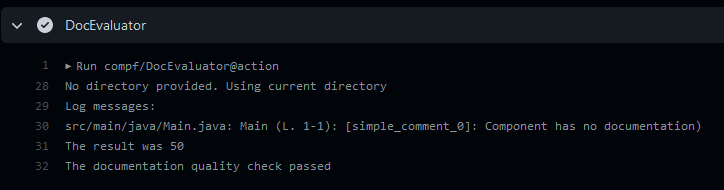
\includegraphics[width=\columnwidth]{figures/appendix/passed.png}
    \caption{Foto vom Tool: Dokumentationsqualität ausreichend}
    \label{fig:passed}
\end{figure}
\begin{figure}[htbp!]
    \centering
    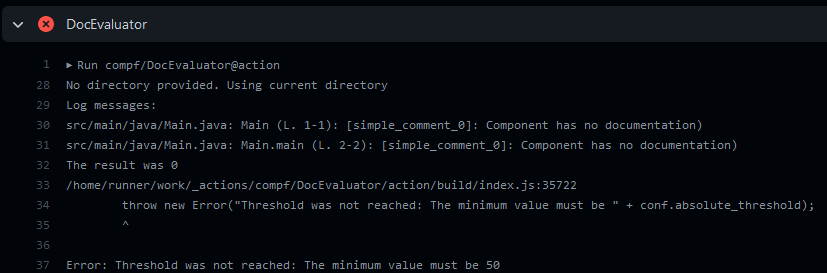
\includegraphics[width=\columnwidth]{figures/appendix/absolute_threshold.png}
    \caption{Foto vom Tool: Dokumentationsqualität zu schlecht}
    \label{fig:absolute}
\end{figure}

\end{appendices}
	



\chapter*{Erklärung zur selbstständigen Abfassung der Masterarbeit}

Ich versichere, dass ich die eingereichte Masterarbeit selbstständig und ohne unerlaubte Hilfe verfasst habe. Anderer als der von mir angegebenen Hilfsmittel und Schriften habe ich mich nicht bedient. Alle wörtlich oder sinngemäß den Schriften anderer Autoren entnommenen Stellen habe ich kenntlich gemacht. \\


\bigskip
\bigskip
\bigskip
\bigskip
\noindent
Osnabrück, 18. Oktober 2018 \\

\bigskip
\bigskip
\bigskip
\bigskip
\noindent
Vorname Nachname
\end{document}

